%written in USA's English
\documentclass[master=cws,masteroption=se,english]{kulemt} % oneside
\setup{% Verwijder de "%" op de volgende lijn bij UTF-8 karakterencodering
  inputenc=utf8,
  title={Fuzzing constraint programming languages}, 
  author={ing. Ruben Kindt},
  promotor={Prof.\, dr.\ Tias Guns},
  assessor={ },
  assistant={Ir. Ignace Bleukx}
}
% Detecting bugs in constraint programming languages
% Fuzz testing constraint programming languages
% Lifting combinatorial fuzz testing for constraint programming languages


% Verwijder de "%" op de volgende lijn als je de kaft wil afdrukken
%\setup{coverpageonly}
% Verwijder de "%" op de volgende lijn als je enkel de eerste pagina's wil
% afdrukken en de rest bv. via Word aanmaken.
%\setup{frontpagesonly}

% Kies de fonts voor de gewone tekst, bv. Latin Modern
\setup{font=lm}

% Hier kun je dan nog andere pakketten laden of eigen definities voorzien
%\usepackage{todonotes}
\usepackage{xcolor}
\usepackage{pifont}   % used for checkmarks
\usepackage{listings} % used for code listings
\usepackage{csquotes} % makes sure that the quotes follow the same typeset as the rest of the text
%\usepackage[tableposition=top]{caption} % caption above table
\usepackage[margin=10pt,font=small,labelfont=bf,labelsep=endash, tableposition=top]{caption}

\usepackage{float}

%thanks to https://github.com/youngkd/MSPSP-InstLib/blob/master/format-description.tex
%----------------------------------------------%
% Syntax highlighting for MiniZinc in listings %
%----------------------------------------------%
\definecolor{ForestGreen}{RGB}{34,106,46}
\usepackage{color}
\lstdefinelanguage{minizinc}{
	morekeywords={
		%% MiniZinc keywords
		%%
		ann, annotation, any, array, assert,
		bool,
		constraint,
		else, elseif, endif, enum, exists,
		float, forall, function,
		if, in, include, int,
		list,
		minimize, maximize,
		of, op, output,
		par, predicate,
		record,
		set, solve, string,
		test, then, tuple, type,
		var,
		where,
		%% MiniZinc functions
		%%
		abort, abs, acosh, array_intersect, array_union,
		array1d, array2d, array3d, array4d, array5d, array6d, asin, assert, atan,
		bool2int,
		card, ceil, combinator, concat, cos, cosh,
		dom, dom_array, dom_size, dominance,
		exp,
		fix, floor,
		index_set, index_set_1of2, index_set_2of2, index_set_1of3, index_set_2of3, index_set_3of3,
		int2float, is_fixed,
		join,
		lb, lb_array, length, let, ln, log, log2, log10,
		min, max,
		pow, product,
		round,
		set2array, show, show_int, show_float, sin, sinh, sqrt, sum,
		tan, tanh, trace,
		ub, and ub_array,
		%% Search keywords
		%%
		bool_search, int_search, seq_search, priority_search,
		%% MiniSearch keywords
		%%
		minisearch, search, while, repeat, next, commit, print, post, sol, scope, time_limit, break, fail
	},
	sensitive=true, % are the keywords case sensitive
	morecomment=[l][\em\color{ForestGreen}]{\%},
	%morecomment=[s]{/*}{*/},
	morestring=[b]",
}
%% Settings for listings
%%
\lstset{ %
	backgroundcolor=\color{lightgray},  % choose the background color; you must add
	% \usepackage{color} or \usepackage{xcolor}
	basicstyle=\scriptsize\ttfamily,    % the size of the fonts that are used for the code
	belowskip=0em,
	breakatwhitespace=false,            % sets if automatic breaks should only happen at whitespace
	breaklines=true,                    % sets automatic line breaking
	captionpos=b,                       % sets the caption-position to bottom
	commentstyle=\color{ForestGreen},   % comment style
	%deletekeywords={...},              % if you want to delete keywords from the given language
	escapeinside={\%*}{*)},             % if you want to add LaTeX within your code
	extendedchars=true,                 % lets you use non-ASCII characters; for 8-bits
	% encodings only, does not work with UTF-8
	frame=single,                       % adds a frame around the code
	keepspaces=true,                    % keeps spaces in text, useful for keeping indentation
	% of code (possibly needs columns=flexible)
	keywordstyle=\bfseries\color{blue}, % keyword style
	language=minizinc,                  % the language of the code
	%morekeywords={*,...},              % if you want to add more keywords to the set
	numbers=left,                       % where to put the line-numbers; possible values are (none, left, right)
	%numbersep=5pt,                     % how far the line-numbers are from the code
	%numberstyle=\tiny\color{Gray},     % the style that is used for the line-numbers
	rulecolor=\color{black},            % if not set, the frame-color may be changed
	% on line-breaks within not-black text (e.g. comments (green here))
	showspaces=false,                   % show spaces everywhere adding particular
	% underscores; it overrides 'showstringspaces'
	showstringspaces=false,             % underline spaces within strings only
	showtabs=false,                     % show tabs within strings adding particular underscores
	%stepnumber=1,                      % the step between two line-numbers. If it's 1, each line will be numbered
	stringstyle=\color{purple},            % string literal style
	tabsize=2,                          % sets default tabsize to 2 spaces
	title=\lstname                      % show the filename of files included with \lstinputlisting;
	% also try caption instead of title
}

%\usepackage[style=numeric,sortcites,sorting=nty,backref,hyperref]{biblatex}
%\usepackage[style=numeric,sortcites,sorting=none,backref,hyperref]{biblatex} % no sort, for finding unused ref
%\nocite{*}  % cite all ref, for finding unused ref
\usepackage{biblatex}
\bibliography{references}

% Tenslotte wordt hyperref gebruikt voor pdf bestanden.
% Dit mag verwijderd worden voor de af te drukken versie.
\usepackage[pdfusetitle,colorlinks,plainpages=false]{hyperref}
\hypersetup{allcolors = black}
%%%%%%%
% Om wat tekst te genereren wordt hier het lipsum pakket gebruikt.
% Bij een echte masterproef heb je dit natuurlijk nooit nodig!
%\IfFileExists{lipsum.sty}%
% {\usepackage{lipsum}\setlipsumdefault{11-13}}%
% {\newcommand{\lipsum}[1][11-13]{\par Hier komt wat tekst: lipsum ##1.\par}}
%%%%%%%
\begin{document}
\begin{preface}
Although this thesis was finished with a strict planning I put onto myself, it was immensely fun to work on. From the destructive nature of fuzzing bugs to the fascinating topic of constraint solving it all interested me and I had not a single moment where I had to push myself to start working on it. But this thesis would not have been possible without the following people.


\noindent Firstly, I would like to thank 
professor dr. Tias Guns for the guidance and the proposal of this fascinating topic,
ir. Ignace Bleukx for answering many questions, intensive thesis meetings, proofreading and the cleverness for coming up with the name of CTORM, 
dr. ir. Jo Devriendt for finding bugs within our bug finder, 
the rest of the CPMpy-team, 
Hakan Kjellerstrand for publishing significant amount examples which we used as seeds,
friends for proofreading and 
family for the support during my further studies.
\end{preface}

\tableofcontents*
\setcounter{tocdepth}{5} % this works wow! Now I have a clean TOC but still the pdf outline in depth

\begin{abstract}
This thesis presents a comparative study between three ways of finding bugs in CPMpy as a use case to examine which techniques are suitable to find bugs in constraint programming languages. 
The first technique builds further on an existing paper to test SMT theories, which this paper converts to be able to test CPMpy with. 
A second technique uses output preserving equivalent changes to see whether the original result differs from the result of the modified program and 
the final technique uses the concept of comparing the results of analog programs in order to detect any differentiations between any of the programs. %\todo{feels bad, unsure what to discuss which you can feel in the txt}

% voordelen automatisch bugs vinden? = not crusial info
% results Abstrakt is suppost to be a sneak peek not a spoiler
%The \texttt{abstract} environment contains a more extensive overview of
%the work. But it should be limited to one page.
\vspace*{\fill}
\noindent
\textbf{Keywords:} Constraint programming, CPMpy, fuzzing, bugs, STORM, differential testing
\end{abstract}

\begin{abstract*}
%
Deze masterproef stelt een vergelijkende studie voor tussen drie manieren om bugs te vinden met CPMpy als voorbeeld. Dit om te onderzoeken welke technieken geschikt zijn om bugs te vinden in programmeertalen voor beperkingen.
De eerste techniek bouwt verder op een bestaande paper om SMT-theorieën te testen via de tester STORM, deze paper converteert STORM naar een tester die om kan gaan met CPMpy om daar dan mee te kunnen testen.
Een tweede techniek maakt gebruikt van resultaatgebonden equivalente wijzigingen om te evalueren of het oorspronkelijke resultaat verschilt van het resultaat van het gewijzigde programma. En ten slotte gebruikt de laatste techniek het concept van gelijkaardige programma's, om de resultaten hiervan te vergelijken om zo eventuele verschillen tussen de programma's te detecteren.

%State of the art 
%'in deze masterproef stellen wij een vergelijkende studie voor om auto bugs te vinden in cpl met als voorbeeld taal de CPMpy written by Tia's Guns at al.
%Voordelen automatisch bugs (Tijdwinst, Safer programma)

\end{abstract*}

% Een lijst van figuren en tabellen is optioneel
%\listoffigures
%\listoftables
% Bij een beperkt aantal figuren en tabellen gebruik je liever het volgende:
\listoffiguresandtables
\lstlistoflistings
% De lijst van symbolen is eveneens optioneel.
% Deze lijst moet wel manueel aangemaakt worden, bv. als volgt:
\chapter{List of Abbreviations and Symbols}
\section*{Abbreviations}
\begin{flushleft}
  \renewcommand{\arraystretch}{1.1}
  \begin{tabularx}{\textwidth}{@{}p{14mm}X@{}}
  	
%Alphabetic pls
	CI/CD & Continuous Integration and Continuous Deployment, a pipeline for newly written code to repeatably be build, test, release, deploy and more. \\
    CP & Constrain Programming language sometimes also referred to as CPL \\
    CPL & Constrain Programming Language also referred to as CP \\
    CNF & Conjunctive Normal Form, which is a boolean formula written using conjunctions of distinctions. \\
    CSP & Constraint Satisfaction Problem is a problem with constraints and variable with a specific domain e.g., boolean, finite and others.\\
    CPMpy & Constraint Programming and Modeling language for Python.\\
    CVC & Cooperating Validity Checker a popular SMT-theorem prover \\
    PUT & Program Under Test, the piece of code, application of program that is tested on for potential bugs. \\
    LLVM & Although it looks like an abbreviation, it is not. LLVM is the name of a project focused on compiler and toolchain technologies. \\
    MIP & Mixed Integer Programming, theory where decision variables are allowed to be integers \\
    MUS & Minimal Unsatisfiable Subset, the smallest subset possible that is not satisfiable \\
    SMT & Satisfiability Modulo Theory \\
    SUT & Software under Test, analogue to PUT \\
  \end{tabularx}
\end{flushleft}

\section*{Symbols}
\begin{flushleft}
  \renewcommand{\arraystretch}{1.1}
  \begin{tabularx}{\textwidth}{@{}p{14mm}X@{}}
 	$\sim$ & negation used by CPMpy\\
 	$\&$ & and used by CPMpy\\
 	$\vert$ & or used by CPMpy\\
  	$\neg$ & logical negation \\
  	$\land$ & logical and \\
  	$\lor$  & logical or \\
  \end{tabularx}
\end{flushleft}

% Nu begint de eigenlijke tekst
\mainmatter

\chapter{Introduction}
\label{cha:intro}
There are a lot of causes for bugs: software complexity, multiple people writing different parts, changing objective goals, misaligned assumptions and more. Most these things can not be avoided during the creation of software but are the cause of program crashes, vulnerabilities or wrong outcomes. Multiple forms of prevention have been created like: the various forms of software testing, documentation, automatic tests and code reviews. All with the aim to prevent the occurrence of bugs and to reduce the cost associated with them. While automatic test cases often evaluate the goals of software end evaluate previous known bugs, it can do much more. Fuzzing software is a part of those automatic tests, a technique that is popular in the security world for exploit prevention. This technique generates random input for a program under test (PUT) and monitors if the program crashes or not. This explanation was the original interpretation of fuzzing as preformed by Miller\cite{4originalFuzzingUnixUtils}, today this technique is seen as random generation based black box fuzzing while the current fuzzing envelops a broader term, as Man\`es et al.\cite{13manes2019survey} put it nicely,
\begin{quote}
"Fuzzing refers to a process of repeatedly running a program with generated inputs that may be syntactically or semantically malformed."
\end{quote}, as quoted from \cite{13manes2019survey}.
With this technique we will try to detect bugs in the constraint programming and modeling library CPMpy \cite{17guns2019increasing} created by Prof. dr. Guns et al.

\todo{modus operandi bij intro}

\section{The usage of fuzzers in the software development cycle}
During the development phase of software, tests are preformed to check if the written code matches the expected and wanted output. This can be done by the developers themselves or by quality assurance testers which do this full time and this on multiple different ways: code review, manual testing or automated testing. Those could exist out of unit tests, checking for known bugs, confirming that the use cases are working, code audits, dynamic testing, fuzzing and others. None of the techniques mentioned above can prevent all possible bugs from occurring on top of that using only a single technique would cost more to find the same level of bugs then using multiple techniques. Sometimes a code audit is better, for example in situations where you want to know something easy that is most likely plainly written in the code. Other cases dynamic testing may be better, image you have a program which parses curricula vitae to check if candidates match the job position and you want to check if fresh Computer science graduates match the position software analyst. In this case it may be a lot easier to simulate the use case than to dive into the code. In situations where you want to test if bugs exist, you may not know where to start inside of the PUT, this is where Fuzzing may be the correct tool to use. Fuzzing emerged in the academic literature at the start of the nineties, while the industry's full adoption thirty years later is still ongoing. Multiple companies like Google, Microsoft and LLVM have created their own fuzzers and this together with a pushing security sector for the adoption has caused fuzzing to become a part of the growing toolchain for software verification.

\section{Fuzzing and security}
The adoption of fuzzers has definitely gained speed due to its proven effectiveness in finding security exploits. For example ShellShock, Heartbleed, Log4Shell, Foreshadow and KRACK could have been found using fuzz testing as shown in multiple sources \cite{ShellShockViaFuzzing}, \cite{HeartbleedViaFuzzing}, \cite{Log4ShellViaFuzzing}, \cite{34ForeshadowViaFuzz} and fuzzing is even recommended by the authors to prevent similar exploits \cite{33KrackViaFuzz} and \cite{35ForeshadowFuzzRecom}.

\section{Constraint programming in general}
%	what is CP and family, differences, \cite{freuder1997pursuit}
%	usage
%	what could go wrong, cost of bugs

\section{CPMpy}
%	section on how CPMpy works and convorts for other solvers \cite{CP2021 Tutorial "CPMpy, a Numpy-based CP Modeling Environment} and \cite{https://github.com/CPMpy/cpmpy/} and where errors could occure, whitch ones are in/out of scope

\section{fuzzing history}
% why fuzzing, ref to securrity and \cite{25MillerOnMacOS} examples of viruese
%bit of history around fuzzing or CP
% first study in fall of 1988 paper in 1990
% miller 2020 heeft hiervoor de start aan bronnen, pagina 2 middel of linker kolomn
%	generation based, mutation based | White gray, back box | directed fuzzing, coverage-based fuzzing \cite{11Fuzzingasurvey}


%%% Local Variables: 
%%% mode: latex
%%% TeX-master: "thesis"
%%% End: 

\chapter{Fuzzing}
\label{cha:2:fuzzing}
\label{cha:2:intro}
The rise of fuzzing came with Miller giving a classroom assignment\cite{21FuzzingAssignment} in 1988 to his computer science students to test Unix utilities with randomly generated inputs with the goal to break the utilities. Two years later in December he wrote a paper\cite{4originalFuzzingUnixUtils} about the remarkable results, that more than 24\% to 33\% of the programs tested crashed.
In the last thirty years the technique of fuzzing has changed significantly and various innovations have come forward. In this chapter we will look at classifications made, what the fuzzer expects as input, what we can expect as output and we will look at the most popular fuzzers.

\section{Classifications}
\label{cha:2:Classifications}
The three most popular classifications are\cite{12Fuzzingasurvey}\cite{13manes2019survey}\cite{30FuzzingHackartandscience}: how does the fuzzer create input, how well is the input structured and does the fuzzer have knowledge of the program under test (PUT)?

\subsection{Generation and mutation}
\label{cha:2:generationMutation}
A fuzzer can construct inputs for a PUT in two ways, it can generate input itself or it can take an existing input, called seeds, and modify them. While Generation is more common when it comes to smaller inputs, the opposite is true for larger inputs where modification has the upper hand. This is cause by the fact that generating semi-valid input becomes a lot harder the longer the input becomes. For example, generating the word "Fuzzing" by uniformly random sampling ASCII, has a chance of one in $5*10^{14}$ of happening, making this technique infeasible when we want to generate bigger semi-valid inputs. With mutation we can start with larger and already valid input and make modifications to create semi-valid inputs. With this last technique the diversity of the seeding inputs does become quite important. Ideally we would have an unlimited diverse set of inputs, but due to limited computation and available inputs we sometimes need to take a subset. In a paper by Alexandre Rebert et al. \cite{14rebert2014seedselecting} they propose that seed selection algorithms can improve results and compare random seed selection to the minimal subset of seeds with the highest code coverage among other algorithms. 

\subsection{Input structure}
\label{cha:2:InputStructure}
%lexical, sementical, constraint or random
While we have discussed the bigger scope on how inputs are created, let us go into more detail; as we have seen before, fuzzing started with Miller's classroom assignment. This random generation of inputs falls under 'dumb' fuzzing due to only seeing the input as one long list of independent symbols with no knowledge of any structure. This technique can be applied similarly to mutational fuzzing as well, compared to only adding symbols with generational fuzzing here we also remove or change randomly selected symbols. 
We can create three types of inputs: non-valid semi-valid and valid inputs. With non-valid inputs we will almost be exclusively testing the syntactic stage of the PUT, often called the parser. Either the input crashes the parser or it will be detected as invalid by the parser and the PUT will stop running. With semi-valid inputs we hope to be as close as possible to valid inputs in order to explore beyond the parser and to catch bugs deeper in the PUT. And lastly with valid input we are testing if the PUT behaves as expected and does not crashes.
A smarter technique is referred to techniques, which have knowledge about the structure inputs can or should have. This increases the chance of inputs passing the parser and being able to test the deeper parts of the PUT, this at the cost of needing an increased complex fuzzer. We can build a 'smart' fuzzer by adding knowledge about keywords (making it a lexical fuzzer) or by adding knowledge about syntax (for a syntactical fuzzer, which can for example match all parentheses). Directed fuzz testing, where we guide the fuzzer on a specific path, does fit in this category of a 'smart' fuzzer as well but it is not possible in a black box environment, more on that in the next section.

\subsection{Black, gray and white box fuzzing}
\label{cha:2:BlackGrayWhiteFuzzing}
Now that we have discussed adding knowledge of inputs to the fuzzer, we can also add knowledge about the PUT to the fuzzer. Which brings us to black, gray and white box fuzzing. With black box fuzzing we have no knowledge about the inner working of the PUT and we treat the PUT as a literal black box, we provide input and we look at what comes out. With this minimal information the fuzzer then tries to improve its input creation. Compared to black box fuzzing, gray box fuzzing usually comes with tools that give indirect information to the fuzzer. Tools like: code coverage, timings, classes of errors as measurements are all used as feedback, but more measurements are possible. Lastly, as you may have predicted, white box testing is the term used when the fuzzer has as much information to it available as possible. It will have access to the source code and can adjust their inputs to fuzz specific parts of the code (this falls under directed fuzzing). White box fuzzing does have a higher computation cost due to having to reverse engineer the path to specific edge cases, meaning that it can find more bugs per input but creating those inputs takes more time compared to black box fuzzing. The differentiation between black, gray and white box fuzzing is not clear cut, most people would agree that white box fuzzing has full knowledge about the PUT, including the source code, that gray box fuzzing has some knowledge about the PUT and that black box fuzzing has little to no knowledge about the PUT. Going into more detail, all we can say is that it is no longer a black-and-white situation and that the lines has become fuzzy. \todo{Ask permission to do this}

\section{Classifying fuzzers}
\label{cha:2:OtherFuzzers}
Now that we know how we can classify fuzzers, let us look at some existing fuzzers to see how they work. For starters Miller's original work, which we discussed earlier, was a random generation based black box fuzzing. And started off as an assignment for his students to test the reliability of Unix utility programs by trying to break them using a fuzz generator, which was able to generate printable ASCII, non-printable ASCII, with or without null terminating characters of a random length. That resulted in a successful paper\cite{4originalFuzzingUnixUtils} two years later. His later work in 1995 on even more UNIX utilities, his work on X-Windows servers\cite{26miller1995fuzzrevisited}, his work in 2000 on Windows NT 4.0 and Windows 2000\cite{24MillerWindows}, his work on MacOS\cite{25MillerOnMacOS} and his later revisit\cite{3miller2020relevanceOfClasicalFuzzTesting} on fuzzing all fall in the same category of random generation based black box fuzzing. This papers showed that a significant portion of programs are able to be crashed with random inputs. Of the programs tested 15 to 43\% of the Unix utilities crashed, 6\% of the open-source GNU utilities crashed, 26\% of X-Window applications crashed, 45\% of Windows NT 4.0 and Windows 2000 programs crashed and 16\% MacOS programs crashed.

A couple of years later, KLEE\cite{8KLEE} was developed by Cadar et al. KLEE is a generation based white box fuzzing tool build with the idea that bugs could be on any code path and that testing should cover as code much as possible. A code coverage tool is used to test which lines of code are executed and this combined with the feedback KLEE got from the symbolic processor and the interpreter it can generate improved inputs. KLEE does this by symbolically executing the program executions branching on any dangerous operations and when it finds an error it will convert the symbolic to a concrete representation based on the constraints it needed to get passed the specific branches and uses this concrete representation to test the original program.With this stride to obtain 100\% code coverage it should be noted that covering a line of code does not mean that line of code has been found to contain no bugs, but not going over lines of code definitely means that the lines remain untested. Therefore code coverage code coverage is sometimes used as a relative metric, checking if a specific test raises the code coverage, means that a test uses a new part of the code base that has not been tested yet. This combined with the fact that getting a high code coverage is a demanding task and does not easily gets to 100\% turns code coverage into a well rounded measurement.

As for the more popular fuzzers, is the American fuzzy lop\footnote{\url{https://github.com/google/AFL}} (AFL), which named after a rabbit breed and is a C and C++ focused mutation based gray box fuzzer released by Google. But due inactivity on Google's part the fork AFL++\footnote{\url{https://github.com/AFLplusplus/AFLplusplus}} has become more popular than the original and is maintained actively by the community\cite{27AFL++}. Not only is it actively maintained, it is also actively used by researchers like: Lennert Wouters who used it to extract SpaceX Startlinks user terminal firmware \footnote{\url{https://www.esat.kuleuven.be/cosic/blog/dumping-and-extracting-the-spacex-starlink-user-terminal-firmware/}}. \todo{watch his talk, read paper}
Not only did AFL spark AFL++, it has also sparked a python\footnote{\url{https://github.com/jwilk/python-afl}} focused version, a Ruby\footnote{\url{https://github.com/richo/afl-ruby}} focused one, a Go\footnote{\url{https://github.com/aflgo/aflgo}} focused version and is shown by Robert Heaton\cite{AFLWrapper} to not be difficult to write a wrapper for it. 

A potential reason to the inactivity of Google on the ALF project could be the development of both Clusterfuzz\footnote{\url{https://google.github.io/clusterfuzz/}} and OSS-fuzz\footnote{\url{https://google.github.io/oss-fuzz/}}, a scalable fuzzing infrastructure and a combination of multiple fuzzers respectively. With the former one being used in OSS-fuzz as a back end to create a distributed execution environment. This with quite a bit of success\cite{31OSS-FuzzBugs},
\begin{quote} \todo{September update this}
	"As of July 2022, OSS-Fuzz has found over 40,500 bugs in 650 open source projects.",
\end{quote} according to the repository itself. 
Not only Google has come forward with a fuzzer. Even Microsoft has jumped on board of fuzzing with OneFuzz\footnote{\url{https://github.com/microsoft/onefuzz}}, a self-hosted Fuzzing-As-A-Service platform which is intended to be integrated with the CI/CD pipeline. Although looking at the given stars on the Github repository, it looks like Google's tools are more popular than Microsoft' ones.
The last prominent fuzzer we are going to take a look at is the LibFuzzer\footnote{\url{https://llvm.org/docs/LibFuzzer.html}} made by LLVM, a generation based gray box fuzzer which is a part of the bigger LLVM project\footnote{\url{https://github.com/llvm/llvm-project/}} with the focus on the C ecosystem. Being in the same ecosystem as AFL, LibFuzzer can be used together with AFL and even share the same seed inputs.

\subsection{Testing CP and SMT with Fuzzers}
Until now we discussed fuzzers more generally, we would like to deliberate specific fuzzers build for testing constraint programming languages (CP) and satisfiability modulo theory (SMT) solvers.


\begin{figure}
	\centering
	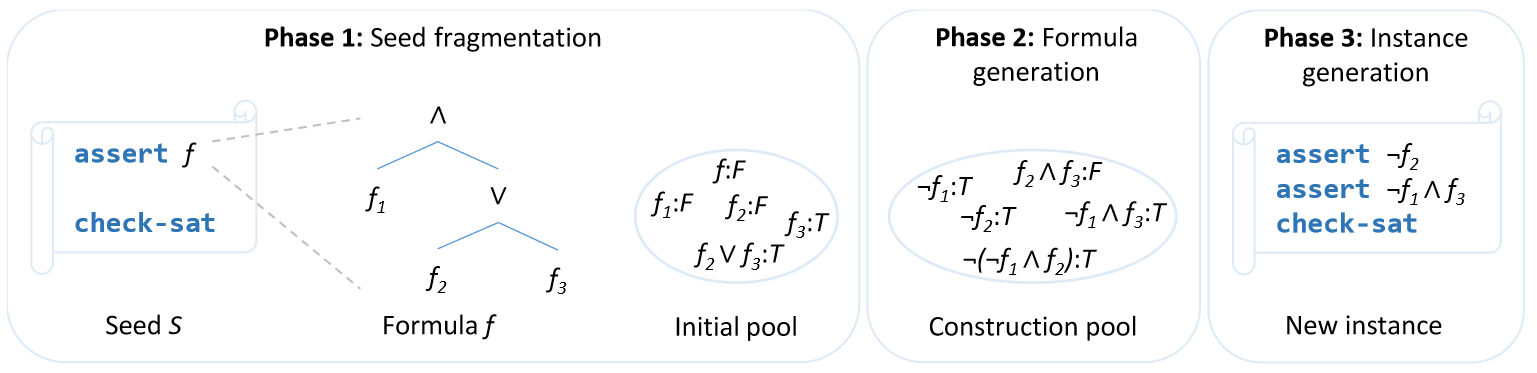
\includegraphics[width=1.0\textwidth]{images/STORM}
	\caption{Overview of the three STORM phases as presented by Muhammad Numair Mansur et al. in "Detecting Critical Bugs in SMT Solvers Using Blackbox Mutational Fuzzing"\cite{1mansur2020detecting}.}
	\label{fig:STORM}
\end{figure}
One of those fuzzers is STORM which is a mutation based black box fuzzer created by Muhammad Numair Mansur et al.\cite{1mansur2020detecting} to find critical bugs in SMT solvers. In their paper they explain the inner working thoroughly, but briefly summarized STORM creates an initial pool of smaller formulas from  existing formulas found in seeds, uses another solver to create models of those smaller formulas. To then construct more complex formulas with the knowledge of their ground truth, with this STORM can test the SMT solver as can be seen in figure \ref{fig:STORM}. This novel way of fuzzing SMT solvers with inputs that are satisfiable by construction and has been cited significantly considering that it is a recent paper.


Another technique for fuzzing SMT solvers is the one proposed by Dominik Winterer et al. with their fuzzer YinYang\cite{43YinYang}, which uses "Semantic Fusion" to test the solvers.
\begin{quote}
	"Our key idea is to fuse two existing equisatisfiable (i.e., both satisfiable or unsatisfiable) formulas into a new formula that combines the structures of its ancestors in a novel manner and preserves the satisfiability by construction. This fused formula is then used for validating SMT solvers."
\end{quote} As quoted from "Validating SMT Solvers via Semantic Fusion"\cite{43YinYang}
Dominik Winterer et al. take a free variable from each of the equisatisfiable formulas to be able to create a new variable using a reversible fusion function. For example a formula $\phi_1$ = X > 10, $\phi_2$ = Y < 9 with the fusion function for Z = X + Y would become $\phi_3$ = Z - Y > 10 $\land$ Z - X < 9, linking both satisfiable formulas together. For unsatisfiable formulas an extra conjunction is needed with the definition of the new variable, because a substitution could result in the loss of the unsatisfiability of the formula as mentioned in the paper. The results of the paper where also significant with 45 bugs in state-of-the-art SMT solvers in Z3\footnote{\url{https://github.com/Z3Prover/z3}} and CVC4\footnote{\url{https://cvc4.github.io/}}. Dominik Winterer et al. also give multiple fusion functions like multiplication and string concatenations which can be applied to integers and real numbers and strings respectively. Extending this technique to other data types or more fusion functions would not be difficult.

\todo{falcon} paper 42 fits well here


\subsection{Types of bugs}
\todo{add different result both say sat but One says 'X=9' other says x="10"}
\label{cha:2:TypesOfBugs}
We can also classify the types of bugs found by the fuzzers, as done in a recent paper\cite{1mansur2020detecting} by Muhammad Numair Mansur et al. being: crashes, wrongly satisfied, wrongly unsatisfied or a hanging PUT. With some of these bugs being less acceptable then others. For example, as Muhammad Numair Mansur et al. describes, a crash is preferred for a constraint programming language (CP) over a wrongly unsatisfied model, since there is no way for the user to know that the solver failed in that last case (except for differentiation testing, more on that later). Meaning that the user will treat the result (wrongly) as correct, compare this to a crash were it is clear that something went wrong. With hanging PUT's the user can not draw incorrect conclusions and with wrongly satisfied models the user can check the model's instances and confirm the result before using it further. This is due to the fact that problems are frequently np-hard meaning they are easy to confirm but hard to solve. For practical reasons we will later change the undecidable and hanging PUT's into timeouts. We know that the types of bugs can be classified in more detail, for example crashes into buffer overflows, invalid memory addressing and so on, but we choose to stay with a more general overview for now. An interesting classification to be added is the knowledge whether or not the bug is in the parser part of the PUT or not. The put could already fail on inputs during the interpretation of the inputs and as discussed we would also like to detect bugs deeper in the PUT. As the authors of "Semantic Fuzzing with Zest"\cite{22SemanticFuzzing} would classify, is the bug in the syntactical or in the semantical part of the program?

\section{The oracle problem}
\label{cha:2:OracleProblem}
% see holy grail
%\cite{11freuder1997pursuitHolyGrail}
\todo{ above thing}
%differential testing with whom? diff on what nr outputs, solutions, hash
%knowing the ground truth (STORM bin and YinYang algeb)
GT = Sat, solver = unsat vs GT = unsat solver = sat

The oracle problem describes the issue of telling if a PUT's output was, given the input, correct or not or as said in "The Oracle Problem in Software Testing: A Survey"\cite{10barr2014oracleProblem} 
\begin{quote}
	"Given an input for a system, the challenge of distinguishing the corresponding desired, correct behavior from potentially incorrect behavior is called the test oracle problem."
\end{quote} by Barr et al.
In their paper they discuss four categories: specified test oracles, derived test oracles, implicit test oracles and the absence of test oracles. The biggest category would be the specified test oracles which contains all the possible encoding of specifications like: modeling languages UML, Event-B and more. Their derived test oracles classification contains all forms of knowledge obtained from documentation on how the program should work or by knowledge of previous versions of the program. The last two oracles categories come down to the use of knowing that crashes are always unwanted and the human oracle like crowdsourcing respectively.

\subsection{Handling the oracle problem}
\label{cha:2:handelingOracelproblem}
Although the approach of by Bugariu and M\"uller in "Automatically testing string solvers"\cite{9bugariu2020automaticallyTestingStringSolvers} falls in the first category mentioned above, their approach is innovative. While most fuzzers either use crashes or differential testing (more on that later) to find bugs, they know the (un)satisfiability of their formulas by the way of they are constructed. For satisfiable formulas they generate trivial formulas and then by satisfiability preserving transformations increase the complexity and for unsatisfiable formulas they use $\neg$ A $\land$ A', with A' being a equivalent formula of A, to create the trivial unsatisfiable formulas. To increase the complexity of those trivial formulas, they again depend on satisfiability preserving transformation. This technique of creating formulas satisfiable by construction has also been applied to SMT solvers by Muhammad Numair Mansur et al. called STORM\cite{1mansur2020detecting} which uses mutational input creation compared to the previous generation based techniques. In the paper the authors dissect all SMT assertions into their sub-formulas and create an initial pool. In this pool the sub-formulas are checked if they satisfy or not and with this knowledge new formulas are created for the population pool with ground truth, from this pool new theories are created and tested. This makes that STORM does not need an oracle to test the entire theory, but only the smaller sub-formulas.
%deze controleert dat de sat is still valid by using another solver as oracle (bij het annoteren van T/F values in the init pool)
% de eerste gebruikt een oracle bij het controleren of dat de equi transformations het model niet breken

\subsection{Differential testing}
\label{cha:2:Differential}
As mentioned above a lot of fuzzers use crashes to detect that the PUT has failed to provide a correct output or when possible use differential testing. This latter one uses a single or multiple analogue programs to test if the PUT gave the same output as the analogue programs. Neither techniques is complete: crash based fuzzing can not detect wrong outputs and differential testing requires that one or multiple analogue programs exits and each with an different implementation to get no overlapping bugs. The latter technique may therefore not always be possible due to the existence of those analogue programs.
\todo{ metamorphic testing}

%somewhere a ref to later chapter input simplification (minimisation differantioation)
\todo{this section}
\section{Opinions against Fuzzing}
\label{cha:2:againstFuzzing}
Unreasonable, why would a person do this, creates unnecessary more work to fix
\cite{39differentialTesting} although has focus on diff testing
this fits well with the types of bugs and with other toolchain
although we have a bias due to writing a dissertation about fuzzing, we think that WE are correct and THEY are wrong, proofs see above + finding bugs/exploits is important

\section{Conclusion}
\label{cha:2:conclusion}
\todo{conclusion}
The final section of the chapter gives an overview of the important results
of this chapter. This implies that the introductory chapter and the
concluding chapter don't need a conclusion.


%%% Local Variables: 
%%% mode: latex
%%% TeX-master: "thesis"
%%% End: 
 % CP, SAT and SMT 
\chapter{Detecting crucial parts in inputs}
\label{inputReduction:intro}
When we detect that the program under test (PUT) crashes, wrongly satisfies, wrongly unsatisfies, hangs or gives the wrong solution on a given input we want to know why it does that. What causes this unwanted output and on what line does the bug occurs. With crashes, a stack trace and some luck this could be easy, but when a bug causes a crash in another place or we get another unwanted output the developer may need to debug deep into the code to find the bug. This with a potential large inputs could be a tedious and long assignment, for this reason we would like to know what parts of the input are relevant for the bug. We will discover this further in this chapter, starting with deobfuscating inputs.

\todo{cont here}
\section{Deobfuscating inputs}
\label{inputReduction:Deobfuscating}
\begin{quote}
	"Often people who encounter a bug spend a lot of time investigating which changes to the input file will make the bug go away and which changes will not affect it." 
	\newline
	-Richard Stallman and Ralf Hildebrandt in "Simplifying and Isolating Failure-Inducing Input" \cite{5zeller2002simplifyingIsolatingFailure-inducing}.
\end{quote} 
When receiving a big input the chance of it having parts unrelated to the bug is almost guaranteed, we will call these inputs (unintentionally) obfuscated inputs. Deobfuscating those inputs can take a lot of try and error to see which variations still reveal the bugs or having to walk through the execution to find the bugs. Both take a while if we want to go to absolute minimal inputs, but for developers it is not needed to go to that extreme. As long as we take the bulk of the unrelated parts of inputs away it will help the developer to find the bug faster. With these techniques we can also group similar bugs and duplicate errors (more on that later) which is also fairly useful information for developers.
\subsection{Simplifying}
\label{inputReduction:Simplifying}
To find crucial parts of inputs, it is often achieved either with simplification or Isolation. 
Simplification is the technique where we repeatably remove parts of a failing input and check if it still fails and it often called "delta-debugging", which belongs to the divide-and-conquer family of algorithms \cite{2FuzzingAndDeltaDebuggingSMTSolvers}. 
The algorithm can be seen in figure \ref{fig:ddmin} with 
"$ c_{\mbox{\ding{56}}} $"  %c_X
meaning the failing input to be deobfuscated,
"\ding{52}" %checkmark 
meaning that a test passed with the given input,
"\ding{56}" %cross 
failed with the given input, 
"$\Delta$" and "$\nabla$" being a subset of the input and the complement of the former and
"1-minimal" meaning that not a single character can can change without the input going from failing to passing. Firstly we start the algorithm with the input and a split (n) of two. If there is a subset that still fails on it own, then we continue with that subset else we look for a subset where the complement of the input still fails but where a subsets is missing from the input. In the case where we split the input in two parts this would be the same as te previous. In case we do not find any smaller subset to continue on, then we reduce de granularity of the split by two. To finally when it is no longer possible to remove any part of the input we have obtained an input where all parts are necessary to expose the bug. This input is at the same time also the shortest possible input to trigger this bug, making finding the bug for the developer easier than in the original input filled with unrelated parts. 
An example of delta-debugging to minimize input can be found in figure \ref{fig:ddminExample}. In the first two steps no removal of any part nor complement was possible therefore we reduces the granularity, after which a removal of parts 3 and 4 was found possible. To then use some previous knowledge (lines 9, 10 and 11) with 2 new tests to remove parts 5 and 6). To then decrease the granularity again until we reach a minimal input.

\begin{figure}
	\centering
	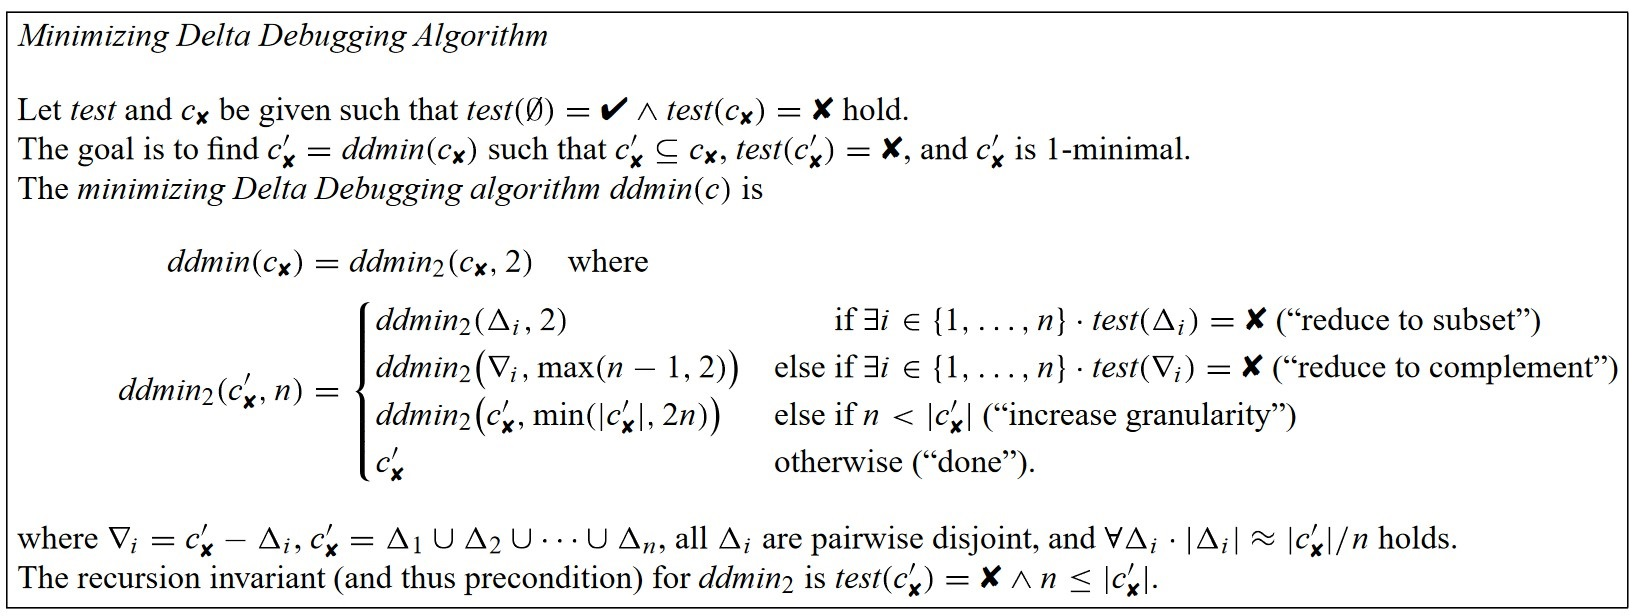
\includegraphics[width=1.0\textwidth]{images/ddminFromPaper5edit}
	\caption{A minimizing delta-debugging algorithm as shown in \cite{5zeller2002simplifyingIsolatingFailure-inducing}.}
	\label{fig:ddmin}
\end{figure}

\begin{figure}
	\centering
	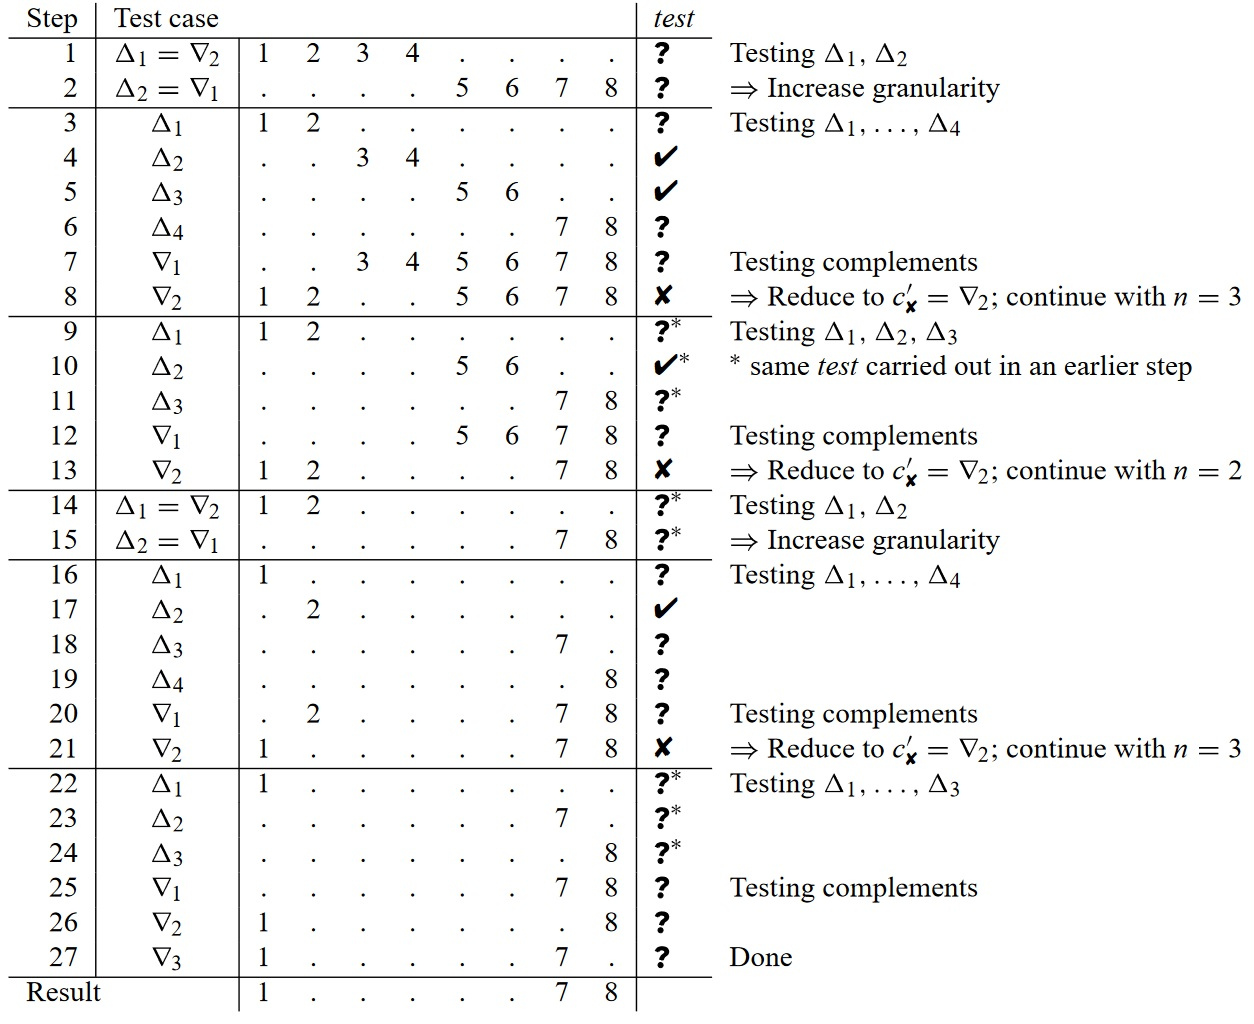
\includegraphics[width=1.0\textwidth]{images/ddminExampleFromPaper5}
	\caption{A minimizing delta-debugging example as shown in \cite{5zeller2002simplifyingIsolatingFailure-inducing} with an input that is deobfuscated with the ddmin() algorithm\ref{fig:ddmin}.}
	\label{fig:ddminExample}
\end{figure}

\subsection{Isolation}
\label{inputReduction:Isolation}
The second technique, isolation, is a technique where instead of minimizing the input we try to find the smallest difference between an input that shows the bug versus an input that does not show the bug. This with the advantage that no matter if we find the bug or not the difference will diminish, either the maximum input will shrink or the minimum input will grow. 
This technique brings extra complexity with the tracking of multiple inputs and bigger inputs often take longer, but according to Andreas Zeller et al. \cite{5zeller2002simplifyingIsolatingFailure-inducing} this is the faster one to the two techniques. 
Figure \ref{fig:simplificationIsolation} shows the difference between simplifying and isolation both finding the critical part of the input. With simplification the critical part is indicated by the last test in the figure while with isolation it is the difference of the last passed and last failed tests.
\begin{figure}
	\centering
	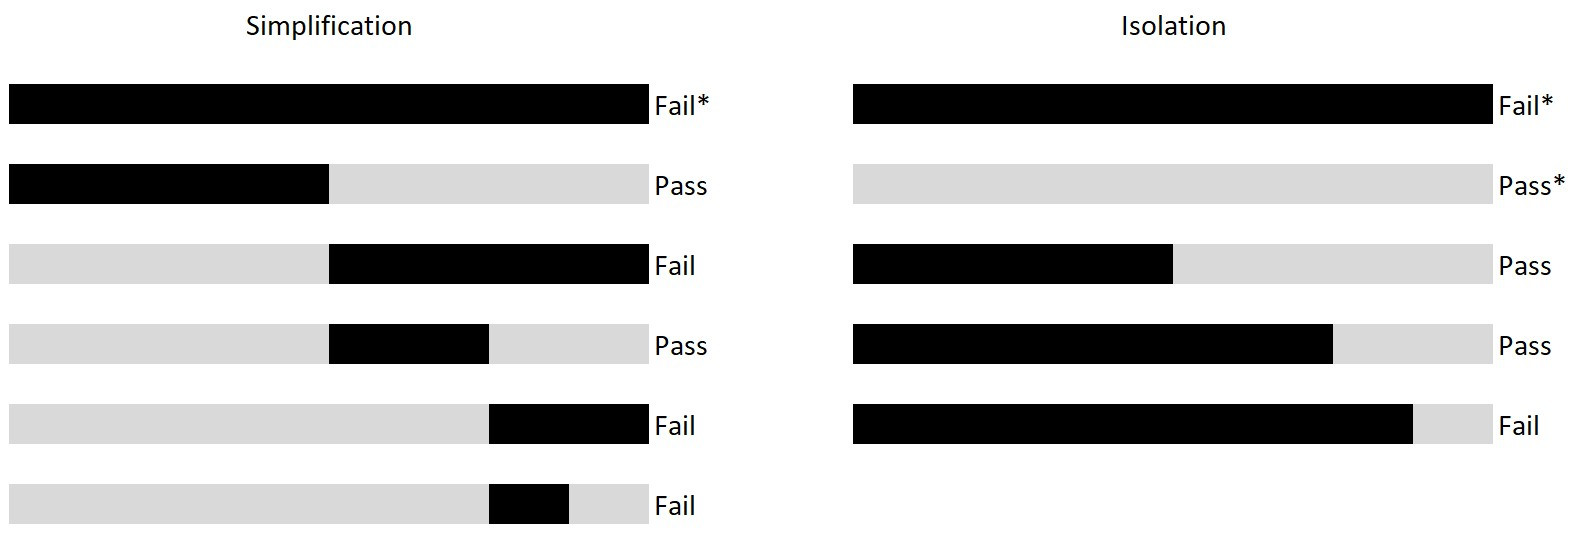
\includegraphics[width=1.0\textwidth]{images/simplificationIsolation}
	\caption{Deobfuscating inputs based on simplification (left) and isolation (right) on the same input. The '*' indicates that the result is already known and does not need to be recalculated. Figure based on an illustrations found in Why programs fail: a guide to systematic debugging by Andreas Zeller \cite{bookZellerwhyProgramsFail}.}
	\label{fig:simplificationIsolation}
\end{figure}

\subsection{Connection with minimal unsatisfiable subset and maximally satisfiable subsets}
\label{inputReduction:MUS/MSS}
For readers that are familiar with the SMT of constraint solving-world will have noticed that this techniques feels similar to a way of finding the minimal unsatisfiable subset (MUS), which it is in the case of a solver (wrongly) stating that an input is unsatisfiable. With MUS you try to find the smallest subset of formulas (or constraints) that will result in an unsatisfiable solution while with MSS you would be trying to find the biggest set of formulas (or constraints) that would result in a satisfiable solution. Both are an iterative process and can be applied in the simplification and the isolation process. But solving which combination of formulas results in the smallest of biggest subset is an computationally intensive progress. Fortunately a lot ot though has already been put in it to reduce it, for example Mark H. Liffiton et al. have proposed multiple "Algorithms for Computing Minimal Unsatisfiable Subsets of Constraints" \cite{51liffiton2008algorithms}. Again we should note that an Minimal input is not needed as we aim to reduces de input to help de developer find the error faster, a difference between a smaller and the absolute minimum will cause for a big difference in practice.

\subsection{Alternative approach}
\label{inputReduction:alt2deobfuscating}
An alternative approach compared to the already mentioned techniques is one by Alexandra Bugariu and Peter M\"uller \cite{9bugariu2020automaticallyTestingStringSolvers} is to forgo the need of deobfuscating inputs by generating inputs "small by construction". Because the smaller the inputs are the space there is for remaining stuff to obfuscate the Input. On the other hand the chance of finding bigger bugs with multiple constraints interacting with each other will be harder to find.
A last alternative approach would be retrying fuzzing by adding an increasing size limitation to find the same bug input as done by Muhammad Numair Mansur et al \cite{1mansur2020detecting}.

\section{What size to change}
\label{inputReduction:Chucksize}
A subject we glossed over is the chuck size, the size to remove while trying to find the critical parts of the inputs. 
The previous seen techniques will work well on the original fuzz testing by Miller et al. \cite{4originalFuzzingUnixUtils} since those random generated symbols where independent from each other. But when testing more complex words like function names we no longer can split on all possible places, since the input would most likely no longer parse. 
In figure \ref{fig:simplificationIsolation} we conveniently took one-eighth of the input as the chuck sizes for the ease of the example. For performance reasons we hope we can keep our chuck sizes as big as possible to be able to discard larger unrelated parts of the inputs. But when this is not possible we will need to decrease the granularity of the chuck sizes.
For example, to be able to find the critical parts of an input of the form "XXooXooXXoo" (with 'o' being the critical parts and the 'X' being unrelated to the bug) we should always search further with same granularity while the removed parts are already removed until all options with that granularity are searched \cite{bookZellerwhyProgramsFail}. This will make sure that we eliminate all unrelated parts with the specific granularity and get "ooXoooo" instead of "ooXooXXoo". 

For more complex inputs we can apply techniques seen in section \ref{fuzzing:InputStructure} where we discussed the creation of randomly and smarter created inputs. Instead of removing (hopefully) unrelated parts based purely on where the part sits in the input, we can use knowledge of the input structure or knowledge of the PUT to guide us in the removal \cite{bookZellerwhyProgramsFail}. Both lexical (the meaning of words) and syntactical knowledge (the meaning of combinations of words) can be used to help us in deobfuscating complex inputs. Where syntactical knowledge would help us remove the most since it is the bigger of the two.

\subsection{Preserving satisfiability}
\label{inputReduction:preservingSat}
With the techniques as mentioned in section \ref{cha:2:handelingOracelproblem}, "satisfiable by construction" formed inputs will need to take the extra complexity of preserving the ground truth in mind when deobfuscating inputs. When the ground truth says that an input should be unsat and the PUT says it is a satisfiable problem with the following output, then we can not remove constraints to retest if that specific constraint was the cause without knowing the new ground truth. As potential change, this could switch the original input from an unsatisfiable to a satisfiable problem. We could use a trusted solver to make sure that we only retest unsat inputs by retesting each change. or as done by  Muhammad Numair Mansur et al.'s \cite{1mansur2020detecting} technique of trying to fuzz the same seed in the hope to find a smaller input that gives the same bug. Or use other SMT solvers to make sure that the ground truth does not change as Brummayer and Biere \cite{2FuzzingAndDeltaDebuggingSMTSolvers} did.
In the other scenario when he ground truth says that an input should be sat with X amount of models and the PUT says that the input is unsatisfiable. Then we have more options to deobfuscate the inputs. We can use the previously mentioned techniques like the other scenario but we can also use simplifying, isolation, MUS, MSS and the technique of refuzzing like STORM while still preserving the (un)satisfiability of the problem.

\section{The precision effect}
\label{inputReduction:PersisionEffect}
This finding of the same bug needs to be done carefully, so that we do not change a null pointer dereference bug to a parser related bug. This, as discussed in the previous chapter, is because we value some bugs with more importance than others. 
In a paper by Andreas Zeller and Ralf Hildebrandt \cite{5zeller2002simplifyingIsolatingFailure-inducing} they talk about this exact problem which they called "the Precision Effect". Sometimes this is not a problem, for example when we are trying to find all possible bugs and will rerun the fuzzer after each incremental improvement or the situation where a deeper bug turns into another deep bug. But overall we try to avoid this effect, which can be done with the techniques in the following section.

\section{Deduplication}
\label{inputReduction:Deduplication}
With deobfuscating the inputs we can detect exact copies, but depending on the deobfuscation's time complexity other techniques could be better with similar results. In case where we would have access to stack traces (via crashes) we could differentiate the bugs on the basis of the hash from the backtrace, sometimes even numerous hashes per input depending on the amount of backtrace lines taken. This technique is called "stack backtrace hashing" and is quite popular according to Valentin J.M. Man\`es et al. \cite{13manes2019survey} 
Another technique talked about in that paper, is looking at the code coverage generated by the inputs where the executed path (or hash of it) is used as a fingerprint of the inputs. A technique, used by Microsoft \cite{36semanticsAwareDeduplicationRETracer} is called "semantics based deduplication", where instead of backtrace they use memory dumps to hopefully find the origins of bugs. This use of dumps is less ideal due to traces having more information, but the latter is not always possible due to the performance overhead and privacy causes as specified in the paper. 
A last technique would be looking at the bug description left by manual bug reports, although this dependence on the quality of bug reports and is most likely poorly automatable. 
None of the techniques mentioned above are perfect: with stack backtrace hashing you need access to the backtrace, with coverage some inputs will generate extra function calls and the semantics based deduplication are limited to X86 or x86-64 code with the binary file and the debug information. Neither of those first techniques will work with black box fuzzing unfortunately.

\section{Conclusion}
\label{inputReduction:Conclusion}
In this chapter we discussed why a reduced failing input would be convenient for the further process, what advantages it brings with it while fuzzing PUTs. We have seen multiple methods of deobfuscating inputs from the straightforward simplifying to the heavier isolation. We also looked at state of the art approaches, how they preserve satisfiability and how to avoid having to deobfuscate inputs in the first place. To then end with the advantage of short deobfuscated inputs to prevent duplicates bugs.

%%% Local Variables: 
%%% mode: latex
%%% TeX-master: "thesis"
%%% End: 
 % Fuzzing
\chapter{Result}
\label{cha:4}
\todo{intro ch 4}

% own results 
% comparision with other fuzzers

\section{The First Topic of this Chapter}
\lipsum[78]


\section{Figures}
Figures are used to add illustrations to the text. The \fref{fig:logo} shows
the KU~Leuven logo as an illustration.
\begin{figure}
	\centering
	
\includegraphics{logokul}
	\caption{The KU~Leuven logo.}
	\label{fig:logo}
\end{figure}

\section{Tables}
Tables are used to present data neatly arranged. A table is normally
not a spreadsheet! Compare \tref{tab:wrong} en \tref{tab:ok}: which table do
you prefer?

\begin{table}
	\centering
	\begin{tabular}{||l|lr||} \hline
		gnats     & gram      & \$13.65 \\ \cline{2-3}
		& each      & .01 \\ \hline
		gnu       & stuffed   & 92.50 \\ \cline{1-1} \cline{3-3}
		emu       &           & 33.33 \\ \hline
		armadillo & frozen    & 8.99 \\ \hline
	\end{tabular}
	\caption{A table with the wrong layout.}
	\label{tab:wrong}
\end{table}

\begin{table}
	\centering
	\begin{tabular}{@{}llr@{}} \toprule
		\multicolumn{2}{c}{Item} \\ \cmidrule(r){1-2}
		Animal    & Description & Price (\$)\\ \midrule
		Gnat      & per gram    & 13.65 \\
		& each        & 0.01 \\
		Gnu       & stuffed     & 92.50 \\
		Emu       & stuffed     & 33.33 \\
		Armadillo & frozen      & 8.99 \\ \bottomrule
	\end{tabular}
	\caption{A table with the correct layout.}
	\label{tab:ok}
\end{table}


\section{Conclusion}
The final section of the chapter gives an overview of the important results
of this chapter. This implies that the introductory chapter and the
concluding chapter don't need a conclusion.

%%% Local Variables: 
%%% mode: latex
%%% TeX-master: "thesis"
%%% End: 
 % Detecting crucial parts in inputs
%\chapter{Research questions}
\label{cha:RQ}
\label{RQ:intro}
In this chapter we will discuss the problem we are facing today and where our focus will be when answering the research questions in this dissertation. \todo{Add this chapter to Goals of introductuion}

\section{Problem statement}
\label{RQ:ProblemStatment}
As described in at the introduction of chapter \ref{intro:intro}, bugs are practically unavoidable and always unwanted, especially when a user trusts a program to give a correct answer and it does not. With solvers surrounding constraint programming languages being executed more and more we would like to strongly avoid any bugs in the real world from arising. To this end it would be interesting to find bugs during development without much overhead, a modern approach would be the use of fuzzers. which we will try out on a constraint programming language.

\section{Research questions}
\label{RQ:RQ's}
As the title of the dissertation already may have spoiled it, we are trying out multiple fuzzing techniques out on CPMpy, with the goal of finding which technique works well for this specific type of programming language. This in order to give a push to identify ways of automatically discovering (and maybe solving) new bugs in constrain programming languages. We put forward two regions of research questions we will to focus on.

%\todo{reduce nb of RQ}
\subsection{Main focus: fuzzing technique-focused}
The first and our main focus will be comparing different fuzzing techniques: we are going to modify a successful SMT fuzzer STORM to the CPMpy language, try differential testing between the multiple solvers and out last technique is the use of metamorphic testing. Resulting in the following questions: \newline
Research question 1: What fuzzing technique will find the most bugs? \newline 
Research question 2: What fuzzing technique will find the most critical bugs? \newline
Research question 3: What type of bugs will be found by each fuzzing technique? \newline
%\subsubsection{subfocuses}
%Research question 4: Which metamorphic transformation find the most (critical) bugs? \newline
%focused on: \\
%bool, int, list, array

%\subsection{Solver-focused}
%A second focus we have goes more towards the different solvers and the differences between them resulting in. \newline
%Research question 5: Which solver has the most (critical) bugs? \newline

\subsection{Classification-focused}
Our next and last focus will be on the classification of found bugs, giving us the following research questions. \newline
%To then end with focus three based around the classification of found bugs, giving us the following research questions. \newline
Research question 4: How many (critical) bugs can we find? \newline
Research question 5: What are the causes of the bugs? \newline
%Research question 8: What are the type of bugs found? \newline

\section{Not focused: efficiency and others}
A keen reader may wonder why we do not focus on efficiency, this would result in more bugs being caught in a smaller timeframe. While perfectly valid to investigate we believe that discovering which techniques works best for CP' has a higher value than on top of the techniques investigated being able to run automatically. The efficiency in CP has already significant research and literature on how to optimize the solvers, which take the most amount execution time compared to the testers.

% all written in Python

\section{Conclusion}
\label{RQ:conclusion}
In this short chapter we have seen the problem which to address and the research questions this dissertation will answer in order to do so.

%%% Local Variables: 
%%% mode: latex
%%% TeX-master: "thesis"
%%% End: 
 % Research questions
\chapter{Research questions}
\label{cha:RQ}
\label{RQ:intro}
In this chapter we will discuss the problem we are facing today and where our focus will be when answering the research questions in this dissertation. \todo{I'm not happy with this chapter, should this even be a chapter?}

\section{Problem statement}
\label{RQ:ProblemStatment}
As described in at the introduction of chapter \ref{intro:intro}, bugs are practically unavoidable and always unwanted, especially when a user trusts a program to give a correct answer and it does not. With solvers surrounding constraint programming languages being executed more and more we would like to strongly avoid any bugs in the real world from arising. To this end it would be interesting to find bugs during development without much overhead, a modern approach would be the use of fuzzers. which we will try out on a constraint programming language.

\todo{Layout RQ's}
\section{Research questions}
\label{RQ:RQ's}
As the title of the dissertation already may have spoiled it, we are trying out multiple fuzzing techniques out on CPMpy, with the goal of finding which technique works well for this specific type of programming language. This in order to give a push to identify ways of automatically discovering (and maybe solving) new bugs in constrain programming languages. We put forward two regions of research questions we will to focus on.

%\todo{reduce nb of RQ}
\subsection{Main focus: fuzzing technique-focused}
The first and our main focus will be comparing different fuzzing techniques: we are going to modify a successful SMT fuzzer STORM to the CPMpy language, try differential testing between the multiple solvers and out last technique is the use of metamorphic testing. Resulting in the following questions: \newline
Research question 1: What fuzzing technique will find the most bugs? \newline 
Research question 2: What fuzzing technique will find the most critical bugs? \newline
Research question 3: What type of bugs will be found by each fuzzing technique? \newline
%\subsubsection{subfocuses}
%Research question 4: Which metamorphic transformation find the most (critical) bugs? \newline
%focused on: \\
%bool, int, list, array

%\subsection{Solver-focused}
%A second focus we have goes more towards the different solvers and the differences between them resulting in. \newline
%Research question 5: Which solver has the most (critical) bugs? \newline

\subsection{Classification-focused}
Our next and last focus will be on the classification of found bugs, giving us the following research questions. \newline
%To then end with focus three based around the classification of found bugs, giving us the following research questions. \newline
Research question 4: How many (critical) bugs can we find? \newline
Research question 5: What are the causes of the bugs? \newline
%Research question 8: What are the type of bugs found? \newline

\section{Not focused: efficiency and others}
A keen reader may wonder why we do not focus on efficiency, this would result in more bugs being caught in a smaller timeframe. While perfectly valid to investigate we believe that discovering which techniques works best for CP' has a higher value than on top of the techniques investigated being able to run automatically. The efficiency in CP has already significant research and literature on how to optimize the solvers, which take the most amount execution time compared to the testers.

% all written in Python

\section{Conclusion}
\label{RQ:conclusion}
In this short chapter we have seen the problem which to address and the research questions this dissertation will answer in order to do so.

%%% Local Variables: 
%%% mode: latex
%%% TeX-master: "thesis"
%%% End: 
 % Implementation
\chapter{Results}
\label{cha:6:res}
\label{res:Intro}
In this chapter we discuss the results of all three of the techniques introduced in previous chapter \ref{cha:5:impl}, we explain how we prevented frequently occurring bugs, discuss a diverse subset of found bugs with more detail. To end the chapter with a classification of all bugs and the reception of the bugs.

% multiple runs due toe randomness, how measured
% comparision with other fuzzers
% why did we (not) do code coverage ?
% timeout on the minizinc, but not on the ortools -> manuel work
% if stoppted before it was done due to timeout solvers didn't agree on the amount of solutions

\section{Running the tests}
\label{res:RunningTests}
\label{res:Specs}
All tests were executed on an Ubuntu 20.04.5 LTS with 8GB RAM, an Intel core i5-3380M capable of 2.90GHz and a V-NAND SSD of 500GB 860 EVO Model MZ-76E500 through a SATA 3 connection. Other software versions used can be found in the first section of the implementation chapter \ref{cha:5:impl}. With each technique taking around a day to three days to run more than the nine thousand seed files once. Note that processing a seed once can mean that variants of that seed were run up to 100 times depending on the technique used.

%time when faults are found?

\subsection{Preventing the same bug from occurring frequently}
%these tools often gave the same error again causing the new bug to be hidden, se choice to catch some of the more prevelent bugs, If some one wishes to rerun (parts) It is best to remove those exceptions in order to see the full output
After initial experimentation we noticed that once a bug was found by any of our techniques, the same bug would occur frequently, but in a different seed causing our resulting logs to be cluttered with duplicate bugs. Although we were well aware of the possibility these duplicate bugs could appear, we underestimated the severity of impact on our workflow. Whereas we planned on using a reactive deduplication technique in post-processing as described in subsection \ref{inputReduction:Deduplication}, after 10.000 occurrences of equivalent bugs, we changed to a preventative approach. 

Once a bug was noted, we tried to prevent it, for crashes this meant adding a try catch for the specific error. While for wrongly (un)satisfiable bugs we looked at special occurrences of keywords in the constraints we knew caused bugs, to then blacklist them. For example, a bug we will discuss in the next section had a specific string of characters, " == 0 == 0". Being able to check the string of characters knowing that it resulted in wrongly unsatisfiable solutions made it possible for us to filter that bug as well. 

Luckily, with these restrictions on the output logs we were able to filter out most duplicate bugs. Naturally this is not an ideal solution, but in this situation it worked well enough. The ideal solution would be that the fuzzer has knowledge of the already found bugs and rejects them. Techniques like these do exist but would bring us too far from the scope of this thesis. Unfortunately, adding strings to blacklists and restarting the tests did result in extra manual overhead.

\section{Results: found bugs}
\label{res:bugs}
%\todo{19 bugs is af h van welke definitie men volgt, met de onze komen we aan 19}
In total we found 19 bugs, three of which were already known in one form or another as an issue. Of those 19 bugs some of them were easy fixes, some were harder and required more time to solve. Depending on which definition of a bug is used, the number of found bugs will differ. With the definition followed in this thesis, a crash, hang or wrong output, 19 bugs remain out of the 22 submitted. At the time of writing not all bugs are resolved (some are just reported days ago). Nevertheless, we are working actively with developers from the CPMpy library to resolve the open bug reports. For now let us look at what we deem to be the most interesting bugs. In order to do this, we will work with the four components we defined earlier in subsection \ref{CP:CPMpy}. This being the model, the transformations, the solver interface and the solvers themselves as seen in figure \ref{fig:4ComponentsOfCPMpy}.


\subsection{Double Negation}
\label{res:bug:DoubleNot}
The first bug we discovered was a bug involving a double negation, a bug where we ask CPMpy to solve the equivalent constraints "X==3" and "not(not(X==3))" at the same time. Given the domain of 'X' contains 3 this solution is trivial. Set variable 'X' equal to 3 and the problem would be satisfied. However not all CPMpy solvers did agree with this, both OR-Tools and Gurobi said that this problem was unsatisfiable through their corresponding CPMpy interface.

This was due to a process within CPMpy responsible for creating a flat normal form. As described by the documentation of CPMpy\footnote{\url{https://cpmpy.readthedocs.io/en/latest/behind_the_scenes.html}} not all solvers interfaced by CPMpy allow an arbitrary nesting of constraints.It is for this reason CPMpy flattens the constraints to what they call 'flat normal form'. With a disclaimer that this definition does not formally exist for CP languages to their knowledge, a statement which we agree with. With this flattened form, CPMpy is able to directly call the solvers or do the last changes needed for the specific solver via the solver interface on the flattened constraints to then send it to the respective solver \cite{CPMpyGithub}. 

Within CPMpy all negations get translated to a comparison with a zero "== 0". Making the double negation turn into a double comparison with zero which was not handled correctly in the normalizing process. Causing a disappearance of a single "not", which in turn resulted in the original constraint converted to the not equivalent constraints "X==3 and not(X==3)". When this gets sent to OR-Tools or Gurobi they correctly answer with unsatisfiable. The other solvers, mainly MiniZinc's subsolvers were not affected by this bug due to not using this normalizing process. Although this normalizing process was subjected to unit tests, these tests contained an incorrect output causing the bug to remain hidden. This bug was only caught using CTORM, due to its frequent use of adding negations and conjunctions. Due to the lack of metamorphic relations containing a double negation this bug was not caught using the metamorphic testing. Neither differential testing caught the bug since no seed had a double "not" in its constraints. 

A showcase of this "double negation" bug can be seen in listing \ref{lst:Bug:DoubleNot}, where a variable 'X' is created on line 3 with a lower bound (lb) of zero and an upper bound of 9 (ub). Then, add the constraint "X == 3" to a created model on line 5 with the "+=" and the same constraint with a double negation on the next line. Remember that CPMpy uses '$\sim$' as a negation. We then see the different solvers solve the same model with a different exit status, unsatisfiable for OR-Tools and Gurobi and feasible for a MiniZinc subsolver. Feasible is a differentiation made by CPMpy within satisfiable with the other option being optimal both explain themselves. This bug report can be found in the GitHub repository issue number \href{https://github.com/CPMpy/cpmpy/issues/142}{142}.


\begin{lstlisting}[language=python, label={lst:Bug:DoubleNot}, caption={The "double negation"-bug.}]
	from cpmpy import *
	
	X = intvar(lb=0, ub=9)
	m = Model()
	m += X == 3
	m += ~(~(X == 3)) # double negation 
	
	m.solve(solver="gurobi")
	print(m.status().exitstatus.name) # UNSATISFIABLE
	
	m.solve(solver="ortools")
	print(m.status().exitstatus.name) # UNSATISFIABLE
	
	m.solve(solver="minizinc:chuffed")
	print(m.status().exitstatus.name) # FEASIBLE	
\end{lstlisting}

The constraints of the Model can be seen in listing \ref{lst:Bug:DoubleNotModelBeforeNorm}. With the variable 'X' on line 2 and both constraints on line 4 and 5. After normalization we can see that we have lost a negation in listing \ref{lst:Bug:DoubleNotModelAfterNorm}. The remaining negation has been put into the equation of "X == 3".

\begin{figure}[h]
	\begin{minipage}{0.5\textwidth}
		\centering
\begin{lstlisting}[language=python, label={lst:Bug:DoubleNotModelBeforeNorm}, caption={The constraints of the "double negation"-bug \emph{before} the normalization process.}]
	Variables:
	X: 0..9
	Constraints:
	X == 3
	X == 3 == 0 == 0
	Objective: None
\end{lstlisting}
	\end{minipage}
	\begin{minipage}{0.5\textwidth}
		\centering
\begin{lstlisting}[language=python, label={lst:Bug:DoubleNotModelAfterNorm}, caption={The resulting constraints of the "double negation"-bug \emph{after} the normalization process.}]
	Variables:
	X: 0..9
	Constraints:
	X == 3
	X != 3
	Objective: None
\end{lstlisting}
	\end{minipage}
\end{figure}



\subsection{Negation of global constraints}
\label{res:bug:NegatedGlobal}
A second bug related to the use of negations were the crashes of the negated global constraints. Where negations of global constraints like \texttt{not(AllDifferent(argList))} would crash with a recursion error. As the normalizing of a negated global constraint would be handled with adding a "== 0" to it. The action of adding a "== 0" to the constraint did not change anything causing the same to happen when the next normalization would be attempted on the global constraint. The solution was to negate the decomposition of the global constraint instead of negating the global constraint, which was suggested in the comments together with a commented out raising of a not-implemented error. The entire function was labeled as work in progress, but the CPMpy-team expected it to work for this use case as they used it in their reification process. The reason it worked in this process was due to a shortcut not being taken, which the negation of global constraints did do, therefore exposing the bug only in the latter case.

It was again due to the normalizing not being used for MiniZinc's subsolvers that the bug only occurred when using OR-Tools and Gurobi as solvers. Moreover, this bug was quickly found by CTORM since it uses a significant number of negations. Due to the metamorphic relation of adding "!= 0" after some constraints the metamorphic tests managed to find it as well. However, it did not get found by our differential tests as no examples negated their global constraints.


A showcase of this bug can be seen in listing \ref{lst:Bug:NotGlobal}, where a variable "pos" is created on line 3 with a shape of 3 meaning that "pos" will be an array of length 3. After creating an empty model, a negation of a global constraint "AllDifferent" is added to a created model on line 5. By negating this constraint, we require the solver to find an assignment to the variables in the array "pos" where at least two have the same value. For example, array "[1 2 2]" would satisfy, but "[1 2 3]" would not. Subsequently, a MiniZinc subsolver is used to solve the problem which returns feasible on respectively line 7 and 8. However, when sending the same to Gurobi it will crash, analogous with the next line if the previous one would not have crashed the program. This bug report can be found in the GitHub repository issue number  \href{https://github.com/CPMpy/cpmpy/issues/143}{143}.


\begin{lstlisting}[language=python, label={lst:Bug:NotGlobal}, caption={The "negation of global constraints"-bug.}]
	from cpmpy import *

	pos = intvar(lb=0, ub=5, shape=3)
	m = Model()
	m += ~AllDifferent(pos)
	
	m.solve("minizinc:chuffed")
	print(m.status().exitstatus.name) # FEASIBLE

	m.solve("gurobi") # crash
	m.solve("ortools") # would crash as well
\end{lstlisting}

\subsection{Power function of Gurobi}
\label{res:bug:Power}
Now we have seen two bugs in the transformation part of CPMpy, which both fit in the transformation component of CPMpy. It is time to look at the solver interface and some bugs we found there. The first one was a bug where the solver Gurobi would crash if we gave a base variable in the power function which had a negative lower bound. Lower bound meaning that the variable was not permitted lower than that specific value. All other solvers would be able to solve "pow(X, 2) == 9" with the variable 'X' defined with a lower bound of -5 and a higher bound of 5. However, Gurobi did not allow this and raised an error as can be seen in listing \ref{lst:Bug:PowGurobi}. This error was then not caught by CPMpy and therefore could not be turned into an error exit status as a result.

This bug was found with the CTORM implementation because there was a seed file which contained this power function with a negative lower bound in the base. However, the solver used to solve this problem was not Gurobi meaning that the bug was not discovered when the example was written. The original example can be found at the CPMpy repository's csplib examples\footnote{\url{https://github.com/CPMpy/cpmpy/blob/b60310d7962bc7631bcf0b9024140e47c1fb302e/examples/csplib/prob005_auto_correlation.py}}. We do not think that CTORM would have found this bug if it was not in the seed file to begin with. This because CTORM does not create new variables nor modifies any bounds of variables. 

The bug was also not found using the metamorphic tests, since no test covered the power function or changed any bounds of variables. Which is not a limitation of metamorphic testing but a limitation of added constraints by us. 
Additionally, since the problem was already in the seed file to begin with, the differential testing did find the bug and logged it. This bug report can be found in the GitHub repository issue number \href{https://github.com/CPMpy/cpmpy/issues/149}{149}.

\begin{lstlisting}[language=python, label={lst:Bug:PowGurobi}, caption={The "power function of Gurobi"-bug.}]
	from cpmpy import *

	m = Model()
	X = intvar(lb=-5, ub=5)
	m += pow(X, 2) == 9

	m.solve(solver="gurobi") # GurobiError
\end{lstlisting}



\subsection{Wrong bound value Error}
\label{res:bug:WrongBounds}
A second bug we found in the solver interface was a missing check on the variable type, this time not in Gurobi but in the PySAT implementation. When checking if a sum of boolean variables matches a specific variable and that variable happens to be an integer instead of a boolean variable causing an error. In this specific case it was a follow-up function still within CPMpy that crashed. This with wrong bounds since it expected a bound of only two possibilities, a boolean variable, but got a larger bound. In all other places we could find a check with an error that would be reported. However, on this spot it was missed, which was quickly patched after reporting it.

Although, CTORM was run with PySAT's subsolvers, it did not find this bug simply due to a check of (un)satisfiability of the original problem at the start of the program. The technique would assume that the original seed was faulty to start with and continue with another solver or another seed. The same happened with the metamorphic tests where we needed to know the (un)satisfiability of the model before the changes, where it would crash again on the original model. Since those crashes were not logged in both techniques, we did not find it with these techniques. The bug did get discovered with the differential tester where each crash did get logged on top of all differences. This bug report can be found in the GitHub repository issue number \href{https://github.com/CPMpy/cpmpy/issues/150}{150}.

%\subsection{Circuit of one} % remove this bug from the txt ?
%\label{res:bug:Circuit}
%On top of bugs related to specific solver or a group of solvers treated differently like the first two bugs. We also found bugs that would be raised unrelated to which solver was used to solve the problem. Which brings us to the bug where we discovered that creating a global constraint, namely circuit, with only one entry would it crash with a not subscriptable error. This bug can be seen as an user caused error and be dismissed, but the CPMpy-team agreed saw it the same way. They marked it as a bug and added a small check.
%
%\todo{which fuzzers found it?}
%
%This bug report can be found in the GitHub repository issue number \href{https://github.com/CPMpy/cpmpy/issues/157}{157}.

\subsection{Naming variables}
\label{res:bug:Naming+andImport}
Now we have seen bugs occur in both the transformations and the solver interface. Let us look at a bug we have found in the model component of CPMpy. 

CPMpy has multiple features like importing, exporting models, adding names variables (not to be confused with the local variables as seen on line 12 in listing \ref{lst:SendMoreMoneyCPMpy}) and more. The adding of the name is to make sure that after an export and import the given variable names are still remembered among other reasons, like to be able to give the solver the variable names. When the programmer does not give a name to a variable as we did on line 12 in listing \ref{lst:SendMoreMoneyCPMpy} with the missing \texttt{name=''} attribute in the \texttt{intvar()} function. Then CPMpy adds a name to the variable without telling the programmer. These variables start with "BV" for boolean variables and "IV" with integer variables and each get appended with their respective incrementing number to prevent similar names. This is because reusing variable names is dangerous as the solvers use this name to differentiate variables from each other.
%\todo{is dit slecht uitgelegd?} Niemand klaagt dus het is leesbaar q:

This brings us to the bug; it occurs when importing a model with automatic naming where those counters did not get updated. Meaning that when a new variable was created with automatic naming it would have an overlapping variable name with a variable that was previously imported. When a solver was then called it would treat both variables as the same resulting in potential wrongly unsatisfiable solutions. The use case is a bit farther from the normal use case a programmer would go through. Nevertheless, this was not considered a misuse of CPMpy according to the developers and at the time of writing a pull request was proposed in which the import function got extended to check the highest occurrence of the boolean and integer counter. This highest occurrence will then be used for the counters of new variables.

An almost related bug is in the naming of variables, when creating them starting with non-alphanumeric symbols like '+', '\%' or others some solvers would crash. Most solvers would happily solve with these names, but MiniZinc crashed with a syntax error when handling the input. Due to the transformation of our model to the text-based Zinc for the subsolver, it can no longer differentiate between the variable name and the code. It therefore crashed when seeing anything that could be interpreted differently than a variable name. MiniZinc does state that identifiers are not allowed to contain special characters, which other solvers and CPMpy do allow. A solution is still being discussed at the time of writing.


In listing \ref{lst:Bug:+} this bug of non-alphanumeric symbols is showcased. With a variable 'i' being declared on line 3 with a lower and higher bound respectively 0 and 5. To then define a name manually and name it '+', this in contrast with the previous listings where CPMpy used automatically naming of the variables.  Due to this non-alphanumeric naming of variables MiniZinc will crash with a syntax error on line 13 while it solved the constraint fine on line 7. Lines 10 and 11 are only added to show what the MiniZinc solver receives which is visible in listing \ref{lst:Bug:+Zinc}. 

\begin{lstlisting}[language=python, label={lst:Bug:+}, caption={A bug showcasing that the naming of CPMpy's variables is less strict than MiniZinc's.}]
	from cpmpy import *
	
	i = intvar(lb=0, ub=5, name="+")
	m = Model()
	m += i > 0
	
	m.solve(solver="ortools")
	print(m.sstatus().exitstatus.name) # OPTIMAL
	
	s = SolverLookup.get("minizinc", m)
	print("".join(map(str, s.mzn_model._code_fragments)))
	
	m.solve(solver="minizinc:chuffed") # crash by syntax error
\end{lstlisting}

\noindent In this second listing (listing \ref{lst:Bug:+Zinc}) we can clearly see that the '+' of line 4 and 5 are out of place syntactically. Which in turn causes the error.

\begin{lstlisting}[language=minizinc, label={lst:Bug:+Zinc}, caption={The resulting Zinc code from listing \ref{lst:Bug:+} used by Minzinc.}]
		% Generated by CPMpy
		include "globals.mzn";
		
		var 3..6: +int;
		constraint (+int) > 4;
\end{lstlisting}

Both of these bugs were not caught by CTORM nor the differential testing, since they do not create new variables. However, the bugs did get caught by the metamorphic testing, the first bug was caught because we imported a seed file where automatic naming was done after which we created a variable too with this process, resulting in the bug. The second one is a bit more embarrassing to write down, as we created a bug in the metamorphic tester which resulted in the (unintentionally) creation of variables starting with a '+'. Our own bug caused us to find a bug in CPMpy. We still label it a caught bug because the automatic bug catcher did find it, although only by a fault we made. These bug reports can be found in the GitHub repository issue number \href{https://github.com/CPMpy/cpmpy/issues/158}{158} and \href{https://github.com/CPMpy/cpmpy/issues/162}{162} respectively.


\subsection{MiniZinc returning zero}
\label{res:bug:MinizincZero}
Our last bug we will discuss in detail was a bug we found with a solver themselves, namely with some MiniZinc subsolver. While solving certain problems with MiniZinc's subsolvers Gecode and others it would sometimes crash with the error that it stopped without output. After reporting it turned out to be a known bug in the MiniZinc Python repository for Windows operating systems and was fixable with setting some path variables correctly. Which CPMpy may solve by adding a warning when this happens or by documenting it.
Given that this problem is an installation problem, all techniques were able to find the bug. This bug report can be found in the GitHub repository issue number \href{https://github.com/CPMpy/cpmpy/issues/156}{156}.

%\subsection{Unsatisfiable Gurobi} % boring bug
%\label{res:bug:UnsatGurobu}
%Our last bug we will discuss is a bug that was found by all three techniques
%
%
%This bug report can be found in the GitHub repository issue number \href{https://github.com/CPMpy/cpmpy/issues/168}{168}.


%\subsection{Solver lookup bug} % boring bug
%\label{res:bug:solverLookup}
%solverlookup() was during development of the tester = manual testing, 

%\todo{optional: bug \href{https://github.com/CPMpy/cpmpy/issues/163}{163} would be a fun explanation for the thesis, but lacks a bug. atm it's a note in \ref{impl:Meta}}


\section{Classifications}
\label{res:Classifications}
Now that we have seen in depth explanations of some bugs, let us give an overview of all found bugs by classifying them based on place, type of the bugs, which solver caused the bugs and which technique found the bugs. The bug number refers to the issue number on GitHub and is a hyperlink to that bug, the second column is a short description of the bug and then the table specific classification follows.

% added above the text that refference it, to prevent tables being back to back
\begin{table}[]
	\centering
	\caption{Table discussing in which CPMpy component the bug was found. With 4 bugs in the model, 7 bugs in the transformations, 7 bugs in the solver interface and one solver bug was found.}
	\label{tab:bug:placeComponent}
	\begin{tabular}{lll}
		\hline
		BugNr & Bug description                                         & Place of the bug \\ \toprule
		\href{https://github.com/CPMpy/cpmpy/issues/142}{142} & double negation gives unsat                            & Transformations \\
		\href{https://github.com/CPMpy/cpmpy/issues/143}{143} & negating global constraints crashes                 & Transformations \\
		\href{https://github.com/CPMpy/cpmpy/issues/145}{145} & solvers lookup crashes                            & Model            \\
		\href{https://github.com/CPMpy/cpmpy/issues/149}{149} & power function with negative lower bound crashes  & Solver interface \\
		\href{https://github.com/CPMpy/cpmpy/issues/150}{150} & wrong bound causes a crash                        & Solver interface \\
		\href{https://github.com/CPMpy/cpmpy/issues/152}{152} & boolean variable does not support implies         & Model            \\
		\href{https://github.com/CPMpy/cpmpy/issues/153}{153} & Gurobi does not run and gave the wrong nr of sol  & Solver interface \\
		\href{https://github.com/CPMpy/cpmpy/issues/154}{154} & JSON Decoder error                                & Solver interface \\
		\href{https://github.com/CPMpy/cpmpy/issues/155}{155} & list has no shape                                 & Solver interface \\
		\href{https://github.com/CPMpy/cpmpy/issues/156}{156} & MiniZinc returns zero causes a crash              & Solver           \\
		\href{https://github.com/CPMpy/cpmpy/issues/157}{157} & circuit of one element crashes                    & Transformations  \\
		\href{https://github.com/CPMpy/cpmpy/issues/158}{158} & identical variable name can cause wrongly unsat   & Model            \\
		\href{https://github.com/CPMpy/cpmpy/issues/159}{159} & unhandled Gurobi exit status 9                    & Solver interface \\
		\href{https://github.com/CPMpy/cpmpy/issues/161}{161} & two separate references for the same variable     & Model            \\
		\href{https://github.com/CPMpy/cpmpy/issues/162}{162} & CPMpy is looser with variable names than MiniZinc & Solver interface \\
		%\href{https://github.com/CPMpy/cpmpy/issues/163}{163} & cyclic expression tree got generated              & Model            \\
		\href{https://github.com/CPMpy/cpmpy/issues/164}{164} & malloc() failure due to unset bounds              & Transformations  \\
		\href{https://github.com/CPMpy/cpmpy/issues/165}{165} & memory violation segmentation fault               & Transformations  \\
		\href{https://github.com/CPMpy/cpmpy/issues/168}{168} & unsatisfiable Gurobi                              & Transformations  \\
		\href{https://github.com/CPMpy/cpmpy/issues/170}{170} & unsatisfiable due to flattening                   & Transformations  \\ \bottomrule        
	\end{tabular}
\end{table}

%\subsection{Place of the bug}
\label{res:PlaceOfBug}
As can be seen in table \ref{tab:bug:placeComponent} the cause of which component failed is well spread out within CPMpy.
With 4 bugs in the model, 7 bugs in the general transformations, 7 bugs in the solver interface and one solver related bug. The one and only solver related bug we found was the one we discussed in subsection \ref{res:bug:MinizincZero}, which was already known by MiniZinc. We would have hoped to find more bugs in the solvers themselves and it was our aim with this thesis. However, either these techniques are not sufficient or most bugs are already found before release or are already reported and solved.

If we look at the reported issues within the GitHub repository of Google's OR-Tools, we find no significant bugs towards the (un)satisfiability or any wrong output by the solver. Which makes us speculate that Google does extensive testing on that front or even has used the techniques used in this thesis. This last one is likely as Google created multiple own fuzzers, which we discussed in subsection  \ref{fuzzing:OtherFuzzers}. Extensive testing is most likely also done by other solvers since they would probably lose reputation if their solver would be proven to not produce the correct result.

%\subsection{What did the bug cause}
\label{res:CauseOfBug}
Like the authors of STORM, we focused with our techniques on the critical faults, this being the wrongly satisfiable, the wrongly unsatisfiable and the wrong number of solutions. Since these critical bugs are harder to detect for the final user than a crash, timeout or other bug. Out of the 19 bugs found 6 of them fall in our category of critical while the other 13 where all crashes as can be seen in table \ref{tab:bug:fault}. Most of those 6 critical bugs were situations where the solver wrongly outputted that a solution was unsatisfiable and there was only one bug where we could find both a wrongly satisfiable and wrongly unsatisfiable solution.

\begin{table}[]
	\caption{Table discussing what type of fault was caused by the bugs.}
	\label{tab:bug:fault}
	\centering
	\begin{tabular}{lll}
		\hline
		BugNr & Bug description                                           & Type of fault   \\ \toprule
		\href{https://github.com/CPMpy/cpmpy/issues/142}{142} & double negation gives unsat                            & wrongly unsat   \\
		\href{https://github.com/CPMpy/cpmpy/issues/143}{143} & negating global constraints crashes                 & crash           \\
		\href{https://github.com/CPMpy/cpmpy/issues/145}{145} & solvers lookup crashes                            & crash           \\
		\href{https://github.com/CPMpy/cpmpy/issues/149}{149} & power function with negative lower bound crashes  & crash           \\
		\href{https://github.com/CPMpy/cpmpy/issues/150}{150} & wrong bound causes a crash                  & crash           \\
		\href{https://github.com/CPMpy/cpmpy/issues/152}{152} & boolean variable does not support implies         & crash           \\
		\href{https://github.com/CPMpy/cpmpy/issues/153}{153} & Gurobi does not run and gave the wrong Nr of sol  & wrong Nr of sol \\
		\href{https://github.com/CPMpy/cpmpy/issues/154}{154} & JSON Decoder error                                & crash           \\
		\href{https://github.com/CPMpy/cpmpy/issues/155}{155} & list has no shape                                 & crash           \\
		\href{https://github.com/CPMpy/cpmpy/issues/156}{156} & MiniZinc returns zero causes a crash              & crash           \\
		\href{https://github.com/CPMpy/cpmpy/issues/157}{157} & circuit of one element crashes                    & crash           \\
		\href{https://github.com/CPMpy/cpmpy/issues/158}{158} & identical variable name can cause wrongly unsat   & wrongly unsat   \\
		\href{https://github.com/CPMpy/cpmpy/issues/159}{159} & unhandled Gurobi exit status 9                    & crash           \\
		\href{https://github.com/CPMpy/cpmpy/issues/161}{161} & two separate references for the same variable     & wrongly unsat   \\
		\href{https://github.com/CPMpy/cpmpy/issues/162}{162} & CPMpy is looser with variable names than MiniZinc & crash           \\
		%\href{https://github.com/CPMpy/cpmpy/issues/163}{163} & cyclic expression tree got generated               & crash           \\
		\href{https://github.com/CPMpy/cpmpy/issues/164}{164} & malloc() failure due to unset bounds              & crash           \\
		\href{https://github.com/CPMpy/cpmpy/issues/165}{165} & memory violation segmentation fault               & crash           \\
		\href{https://github.com/CPMpy/cpmpy/issues/168}{168} & wrongly unsatisfiable Gurobi                      & wrongly unsat   \\
		\href{https://github.com/CPMpy/cpmpy/issues/170}{170} & wrongly (un)satisfiable due to flattening         & wrongly (un)sat \\ \bottomrule
	\end{tabular}
\end{table}

%\subsection{Which solver was responsible for the bug}
\label{res:SolverResponsible}
When looking at table \ref{tab:bug:Solver} we can see which bug was caused by which solver or if it was a solver independent bug. Where we see 5 bugs unrelated to any solver, that OR-tools only occurred together with Gurobi and that OR-Tools and Gurobi didn't share any bugs found with MiniZinc or PySAT. Mainly because OR-Tools and Gurobi share more transformation code than any other solver pair. We also see that Gurobi occurs the most among our bugs, this often due to edge cases on Gurobi's implementation. %Although, it could be coincidental that we found more Gurobi bug than any other we speculate that the software being proprietary makes it less clear-cut to be implemented in CPMpy.

%\begin{minipage}[\textwidth]
\begin{table}[]
	\centering
	\caption{Table discussing which bug was caused by which solver or if it was a solver independent bug.}
	\label{tab:bug:Solver}
	\begin{tabular}{lll}
		\hline
		BugNr & Bug description                                           & Which solver caused it\\ \toprule
		\href{https://github.com/CPMpy/cpmpy/issues/142}{142} & double negation gives unsat                            & OR-Tools and Gurobi          \\
		\href{https://github.com/CPMpy/cpmpy/issues/143}{143} & negating global constraints crashes                 & OR-Tools and Gurobi          \\
		\href{https://github.com/CPMpy/cpmpy/issues/145}{145} & solvers lookup crashes                            & solver independent           \\
		\href{https://github.com/CPMpy/cpmpy/issues/149}{149} & power function with negative lower bound crashes  & Gurobi                       \\
		\href{https://github.com/CPMpy/cpmpy/issues/150}{150} & wrong bound causes a crash                  & all PySAT subsolvers         \\
		\href{https://github.com/CPMpy/cpmpy/issues/152}{152} & boolean variable does not support implies         & solver independent           \\
		\href{https://github.com/CPMpy/cpmpy/issues/153}{153} & Gurobi does not run and gave the wrong nr of sol  & Gurobi                       \\
		\href{https://github.com/CPMpy/cpmpy/issues/154}{154} & JSON Decoder error                                & MiniZinc's subsolver osicbc  \\
		\href{https://github.com/CPMpy/cpmpy/issues/155}{155} & list has no shape                                 & Gurobi                       \\
		\href{https://github.com/CPMpy/cpmpy/issues/156}{156} & MiniZinc returns zero causes a crash              & multiple MiniZinc subsolvers \\
		\href{https://github.com/CPMpy/cpmpy/issues/157}{157} & circuit of one element crashes                    & solver independent           \\
		\href{https://github.com/CPMpy/cpmpy/issues/158}{158} & identical variable name can cause wrongly unsat   & solver independent           \\
		\href{https://github.com/CPMpy/cpmpy/issues/159}{159} & unhandled Gurobi exit status 9                    & Gurobi                       \\
		\href{https://github.com/CPMpy/cpmpy/issues/161}{161} & two separate references for the same variable     & solver independent           \\
		\href{https://github.com/CPMpy/cpmpy/issues/162}{162} & CPMpy is looser with variable names than MiniZinc & all MiniZinc subsolvers      \\
		%\href{https://github.com/CPMpy/cpmpy/issues/163}{163} & cyclic expression tree got generated               & solver independent           \\
		\href{https://github.com/CPMpy/cpmpy/issues/164}{164} & malloc() failure due to unset bounds              & multiple MiniZinc subsolvers \\
		\href{https://github.com/CPMpy/cpmpy/issues/165}{165} & memory violation segmentation fault               & multiple MiniZinc subsolvers \\
		\href{https://github.com/CPMpy/cpmpy/issues/168}{168} & wrongly unsatisfiable Gurobi                      & Gurobi                       \\
		\href{https://github.com/CPMpy/cpmpy/issues/170}{170} & wrongly (un)satisfiable due to flattening         & OR-Tools and Gurobi          \\ \bottomrule
	\end{tabular}
\end{table}
%\end{minipage}

%\subsection{Which technique found the bug}
\label{res:TechniqueToFindBug}
The last table \ref{tab:bug:Technique} shows the techniques finding which bug. CTORM found 10 bugs, metamorphic testing found the most bugs at 13 and differential testing found 11 out of the19 found bugs. This shows that none of the techniques are perfect on their own, in order to find all bugs a combination of techniques would be needed. As the industry's quality assurance processes do for finding bugs in other software packages, where they use a combination of tools as discussed in section \ref{intro:SoftwareDevelopmentCycle}. With a side note that metamorphic testing could come close if more work was put in creating metamorphic relations. Although, this does require creativity and manual labor instead of the other automated techniques.

\begin{table}[]
	\centering
	\caption{Table discussing which technique found the bug. CTORM found 10 bugs, metamorphic testing found the most bugs at 13 and differential testing found 11 out of the 19 found bugs.}
	\label{tab:bug:Technique}
	\begin{tabular}{lllll}
		\hline
		BugNr & Bug description                                           & \multicolumn{3}{c}{\centering  Bug found by} \\ \toprule
		\href{https://github.com/CPMpy/cpmpy/issues/142}{142} & double negation gives unsat                            & ctorm &       &      \\
		\href{https://github.com/CPMpy/cpmpy/issues/143}{143} & negating global constraints crashes                 & ctorm & meta  &      \\
		\href{https://github.com/CPMpy/cpmpy/issues/145}{145} & solvers lookup crashes                            &       &       & diff \\
		\href{https://github.com/CPMpy/cpmpy/issues/149}{149} & power function with negative lower bound crashes  & ctorm &       & diff \\
		\href{https://github.com/CPMpy/cpmpy/issues/150}{150} & wrong bound causes a crash                  &       &       & diff \\
		\href{https://github.com/CPMpy/cpmpy/issues/152}{152} & boolean variable does not support implies         &       & meta  & diff \\
		\href{https://github.com/CPMpy/cpmpy/issues/153}{153} & Gurobi does not run and gave the wrong nr of sol  &       &       & diff \\
		\href{https://github.com/CPMpy/cpmpy/issues/154}{154} & JSON Decoder error                                & ctorm & meta  & diff \\
		\href{https://github.com/CPMpy/cpmpy/issues/155}{155} & list has no shape                                 & ctorm & meta  & diff \\
		\href{https://github.com/CPMpy/cpmpy/issues/156}{156} & MiniZinc returns zero causes a crash              & ctorm & meta  & diff \\
		\href{https://github.com/CPMpy/cpmpy/issues/157}{157} & circuit of one element crashes                    &       & meta  &      \\
		\href{https://github.com/CPMpy/cpmpy/issues/158}{158} & identical variable name can cause wrongly unsat   &       & meta  &      \\
		\href{https://github.com/CPMpy/cpmpy/issues/159}{159} & unhandled Gurobi exit status 9                    & ctorm &       & diff \\
		\href{https://github.com/CPMpy/cpmpy/issues/161}{161} & two separate references for the same variable     & ctorm & meta  &      \\
		\href{https://github.com/CPMpy/cpmpy/issues/162}{162} & CPMpy is looser with variable names than MiniZinc &       & meta  &      \\
		%\href{https://github.com/CPMpy/cpmpy/issues/163}{163} & cyclic expression tree got generated               &       & meta  &      \\
		\href{https://github.com/CPMpy/cpmpy/issues/164}{164} & malloc() failure due to unset bounds              &       & meta  &      \\
		\href{https://github.com/CPMpy/cpmpy/issues/165}{165} & memory violation segmentation fault               &       & meta  & diff \\
		\href{https://github.com/CPMpy/cpmpy/issues/168}{168} & wrongly unsatisfiable Gurobi                      & ctorm & meta  & diff \\
		\href{https://github.com/CPMpy/cpmpy/issues/170}{170} & wrongly (un)satisfiable due to flattening         & ctorm & meta  &      \\ \bottomrule
	\end{tabular}
\end{table}


\section{Reception to the bugs} 
\label{res:ReceptionToBug}
As mentioned in section \ref{fuzzing:OpinionsAgainstFuzzing} there are multiple views on automated bug catching. We could have reported all our found bugs on the issue page of GitHub without further context. Which would have meant more work for the CPMpy-team and then we could perhaps have seen some negative opinions on fuzzing. 
Although we submitted 22 bugs or questions within a time span of 2 weeks with deobfuscating the inputs and some explanation of what happened to get the bug, we saw a grateful welcome. Similar to what was described in the second part of section \ref{fuzzing:OpinionsAgainstFuzzing}. 
For example, the "double negation"-bug\footnote{\url{https://github.com/CPMpy/cpmpy/issues/142}} was called a "serious bug and a great find" and 
the "negation of global constraints"-bug\footnote{\url{https://github.com/CPMpy/cpmpy/issues/143}} was described as an unexpected bug and "another great find".
%\todo{find out if this is useful addition of the thesis?}

%\section{unsat}
%due to the way of importing the file a lot of edge problems become sat or unsat


\section{Conclusion}
\label{res:conclusion}
In this chapter we have seen that the techniques frequently output already found bugs, since none of the techniques have knowledge of already found bugs. However, after filtering previously found bugs the techniques performed well and found 19 bugs in CPMpy. 
We have seen some bugs in detail with most of them already fixed, due to being easily fixable. Most bugs were related to the CPMpy code and only one was responsible for an external solver bug. We suspect this lack of external solver bugs to be caused by well written and tested solvers. We have shown that we found crashes up to critical bugs like wrongly (un)satisfiable solutions and wrong number of solutions with over a variety of solvers. Of all the techniques used, metamorphic testing came just above the other two techniques with 13 found bugs while CTORM found 10 and the differential testing found 11 bugs out of 19. Finally, we noted the grateful welcome of bugs by the CPMpy-team.

%%% Local Variables: 
%%% mode: latex
%%% TeX-master: "thesis"
%%% End: 
 % results
\chapter{Conclusion and future work}
\label{cha:7:conclusion}
\label{con:intro}
In this chapter we will conclude the thesis by discussing the achievements, the limitations of the techniques used and end with possible future work.

\section{Achievements}
\label{con:Achievements}
This thesis achieved to find numerous bugs within CPMpy this with the use of multiple techniques, as discussed in Section \ref{res:Classifications}, some bugs were found by multiple techniques. Out of the 19 bugs found 10 were found by CTORM, 13 by metamorphic and 11 by differential testing, these bugs were mostly found well spread within CPMpy, but very little were found in the solver themselves. A third of the time the bugs resulted in a critical bug, this being wrongly (un)satisfiable or the wrong amount of solutions presented. The other two-thirds of the bugs resulted in a crash. Often caused by smaller edge cases where CPMpy did not follow the specific solver’s specifications, for example the power bug of Gurobi in Section \ref{res:bug:Power}. None of the techniques got a perfect score meaning that when looking for all bugs a combination of tools will need to be made as clarified in Subsection \ref{res:TechniqueToFindBug}. We have also shown that there are multiple techniques to find critical bugs that are not easily spotted otherwise and we have multiple CPMpy specific fuzzing tools.
% addition to other form of testing

The techniques almost achieved semi-automatic testing with the corresponding advantages of ease of use, time savings and more while extensive testing. Both CTORM and differential testing have potential to become fully automatic testing tools after fixing the repeated logging of already found bugs.

%semi automatic more on that later in the next section 
%found metamorphic testing yet to be a bit better compared to the others
%voordelen automatisch testen: tijdswinst, safer program

\section{Limitations}
\label{con:Limitations}
This problem of frequently finding the same bug is a problem, since it clogs the output with repeated or similar bugs, making it harder to find new bugs. The first solution proposed in this thesis was to deduplicate bugs with the technique seen in Subsection \ref{inputReduction:Deduplication}. However, during testing a preventative approach seemed  favorable compared to the reactive approach of filtering out known bugs. Although the filters currently in use work, they require the developer to run a tester, see what the results are and add a try catch for the most occurring bugs. Ideally this manual creation of filters are done automatically by adding the knowledge of the already found bugs to the tester. 

Another limitation to the testers is specifically with the metamorphic testing, in this technique metamorphic relations need to be manually created, these relations are then used to change constraints to an equivalent but different constraint. With more particular relations the technique would have been able to find at minimum the “double negation”-bug and the power bug of Gurobi as well. However, after implementing 30 metamorphic relations creativity for new relations starts to dwindle down. A second limitation will be that these relations will need to be updated or added after each new addition to CPMpy, which results in more work for the developer and another step away from automation.

%add exception once a bug is found for that specific bug and rerunning again manual work
%-> best use during development instead of when a release is wanted. 
%Which may not be a bad way of working.

While working with seeds is better than generating inputs themselves as discussed in Subsection \ref{fuzzing:generationMutation}, it did bring limitations with it. Those limitations being the availability, complexity and diversity of the seeds. For example, the bug with the negation of global constraints was not found using differential testing since none of the over nine thousand seed files had any negation of a global constraint, this was a limitation created by using seed files that originated from examples of CPMpy.

%Another limitation is with the seeds, while we did discuss the advantages of working with self generating inputs compared to using existing inputs in  Where we working with seeds did limit us 
%problems limited by global fucntions of used seeds (somewhat fine),
%diversity of the seed files  

%\subsection{CTORM} NOT USED ATM !
%STORM originated from as a SMT fuzzer, we changed it to be able to handle CP’s 
%but it still modified problem models like it was a SMT; With conjunctions and negations
%Techniques are best applied during development, since Ctorm of to often detects the already found bugs
%only ‘and’ and ‘not’ combinations Just like STORM

%\subsection{Metamorphic testing}
%bug wrong bound would have been found if we logged the crashes of the original file 

%did not find ~(~()) as we didn’t think to check it specifically, we did check ~=0
%all checks ? + combo-able

%meta testing requires extra manual work
%manual written (= work, although not much work), own choice on how complex you make the relations(simple ones work too), still need the creativity, all relations seem to be “why would this crash this is pointless to write” but do crash sometimes

%created cyclic expressions, a bug that was discovered by Jo DeVriendt in bug number \href{www.todo.be}{163}

\section{Future work}
\label{con:FutureWork}
With new code new bugs will appear so the work of a developer will never be done when it comes to finding bugs. Rerunning the techniques could result in even more interesting bugs. 
%new code = new bugs
On top of solving the limitations specified in the previous Section \ref{con:Limitations},
%adding knowledge of already found bugs while searching for the next bug
a look at testing the configuration space would be an interesting addition to the performed study, this testing of configuration space was briefly mentioned in Section \ref{fuzzing:testingWithFuzzers} where the authors of “Fuzzing SMT solvers via two-dimensional input space exploration” \cite{42FalconFuzzingConfigurationSettingsAndNormal} also fuzz test the configuration space of the PUT. For example, there could be bugs that only occur when certain optimizations are turned on or off like: dynamic symmetry breaking or others. Implementing this fuzz testing of the configuration space would definitely be possible within CPMpy as it has directly access to the solvers.
%Which would come closer to what Ignace Bleukx et al. did in \cite{74bleukx2022model}, but instead of speeding up searches we would be trying to find bugs.
%we only did configuration space of the solvers, it may be interesting to know how CP’s including CPMpy react to changes or attributes that tell the solver to solve in a special way 
Finally, an extension to other languages would be possible as a future work as well.

%\section{Conclusion} concluding chapter  doesn’t need a conclusion.

%%% Local Variables: 
%%% mode: latex
%%% TeX-master: “thesis"
%%% End: 
 % conclustion
%\chapter{creation of fuzzer}
\label{cha:x}
\todo{intro ch x}

% own results, multiple runs due toe randomness, how measured
% comparision with other fuzzers

\section{creation of sat and unsat formulas}
see paper 43 p 4
Semantic Fusion
\cite{43YinYang}
een ref to chapter 2

seed files came from the CPMpy repository the main branch and the csplib branch aswell from Hakank's repository downloaded on Tuesday 27/09/2022
Storm downloaded on Tuesday 27/09/2022 from https://github.com/Practical-Formal-Methods/storm 
https://github.com/Practical-Formal-Methods/storm/commit/55d091624523a0544112ffc339fe81103b3daa2b



Storm take in SMT-lib seed files, we can convert them to minizinc and then using fzn2smt but It hasn't been maintained in over a decenta and doing multiple convertions only back could be tricky and would introduce multiple layers which can introduce bugs a normal user would ever see
Therefore we will be refactoring STORM to fit our CPMpy


























%
%\section{Figures}
%Figures are used to add illustrations to the text. The \fref{fig:logo} shows
%the KU~Leuven logo as an illustration.
%\begin{figure}
%	\centering
%	
\includegraphics{logokul}
%	\caption{The KU~Leuven logo.}
%	\label{fig:logo}
%\end{figure}
%
%\section{Tables}
%Tables are used to present data neatly arranged. A table is normally
%not a spreadsheet! Compare \tref{tab:wrong} en \tref{tab:ok}: which table do
%you prefer?
%
%\begin{table}
%	\centering
%	\begin{tabular}{||l|lr||} \hline
%		gnats     & gram      & \$13.65 \\ \cline{2-3}
%		& each      & .01 \\ \hline
%		gnu       & stuffed   & 92.50 \\ \cline{1-1} \cline{3-3}
%		emu       &           & 33.33 \\ \hline
%		armadillo & frozen    & 8.99 \\ \hline
%	\end{tabular}
%	\caption{A table with the wrong layout.}
%	\label{tab:wrong}
%\end{table}
%
%\begin{table}
%	\centering
%	\begin{tabular}{@{}llr@{}} \toprule
%		\multicolumn{2}{c}{Item} \\ \cmidrule(r){1-2}
%		Animal    & Description & Price (\$)\\ \midrule
%		Gnat      & per gram    & 13.65 \\
%		& each        & 0.01 \\
%		Gnu       & stuffed     & 92.50 \\
%		Emu       & stuffed     & 33.33 \\
%		Armadillo & frozen      & 8.99 \\ \bottomrule
%	\end{tabular}
%	\caption{A table with the correct layout.}
%	\label{tab:ok}
%\end{table}
%

\section{Conclusion}
The final section of the chapter gives an overview of the important results
of this chapter. This implies that the introductory chapter and the
concluding chapter don't need a conclusion.

%%% Local Variables: 
%%% mode: latex
%%% TeX-master: "thesis"
%%% End: 
 % futher work ?

% Indien er bijlagen zijn:
%\appendixpage*          % indien gewenst
%\appendix
%\chapter{The First Appendix}
\label{app:A}
Appendices hold useful data which is not essential to understand the work
done in the master's thesis. An example is a (program) source.
An appendix can also have sections as well as figures and references.

\section{Lorem 51}

%%% Local Variables: 
%%% mode: latex
%%% TeX-master: "thesis"
%%% End: 


\backmatter
% Na de bijlagen plaatst men nog de bibliografie.
% Je kan de  standaard "abbrv" bibliografiestijl vervangen door een andere.
%\bibliographystyle{abbrv}
%\bibliography{references}
\nocite{MasterproefRubenKindt}
%\nocite{ThisThesis}
%\nocite{75Chicken} % Easter egg ;)
\printbibliography
\end{document}

%%% Local Variables: 
%%% mode: latex
%%% TeX-master: t
%%% End: 
